\documentclass{bmvc2k}
\usepackage{graphicx}
\usepackage{amsmath}
\usepackage{amssymb}
\usepackage{mathtools} % mathtools builds on and extends amsmath package
\usepackage{algorithm}		% http://ctan.org/pkg/algorithms
\usepackage{algpseudocode}	% http://ctan.org/pkg/algorithmicx% Include other packages here, before hyperref.
\usepackage{comment, url}
%% Enter your paper number here for the review copy
\bmvcreviewcopy{825}

\title{ {\it E}nKCF: Ensemble of Kernelized Correlation Filters for Object Tracking in High Speed}

% Enter the paper's authors in order
% \addauthor{Name}{email/homepage}{INSTITUTION_CODE}
\addauthor{Susan Student}{http://www.vision.inst.ac.uk/~ss}{1}
\addauthor{Petra Prof}{http://www.vision.inst.ac.uk/~pp}{1}
\addauthor{Colin Collaborator}{colin@collaborators.com}{2}

% Enter the institutions
% \addinstitution{Name\\Address}
\addinstitution{
 The Vision Institute\\
 University of Borsetshire\\
 Wimbleham, UK
}
\addinstitution{
 Collaborators, Inc.\\
 123 Park Avenue,\\
 New York, USA
}

\runninghead{Student, Prof, Collaborator}{BMVC Author Guidelines}

% Any macro definitions you would like to include
% These are not defined in the style file, because they don't begin
% with \bmva, so they might conflict with the user's own macros.
% The \bmvaOneDot macro adds a full stop unless there is one in the
% text already.
\def\eg{\emph{e.g}\bmvaOneDot}
\def\Eg{\emph{E.g}\bmvaOneDot}
\def\etal{\emph{et al}\bmvaOneDot}

%-------------------------------------------------------------------------
% Document starts here
\begin{document}

\maketitle

%%%%%%%%% ABSTRACT
\begin{abstract}
Computer vision technologies are very attractive for practical
applications for embedded systems. This is primarily because most of
embedded systems already includes image acquisition pipeline and a
tremendous amount of progresses on research has been made for many
areas in computer vision. However, to successfully deploy a computer
vision algorithm on any existing embedded systems, a vision algorithm
needs to satisfy, at least, two criteria: minimal, manual intervention
after deployment and small footprint of computing resource consumption
and on executable code, with the assumption of reasonably good
performance. To this end, in this paper, we propose an ensemble of the
kernelized correlation filters (KCF), we call {\it E}nKCF, for a
single-target object tracking. In particular, we developed a committee
of KCFs to specifically address the scale-change and dynamic maneuver
of the target over frames. In addition, we devised a Bayes filter for
a smooth transition between individual KCFs' executions. Also, we
slightly modify the {\it E}nKCF to perform tracking in low frame rate
videos dominated by large ego-motion.  large ego-motion.  To verify
the usefulness of the proposed method, we compared the performance of
ours to those of the existing online tracking methods. Experimental
results showed that the performance of ours are 72.53\% for precision
on 20 pixels and 52.90\% for success rate for OTB100 data, and 55.71\%
and 41.71\% for UAV123 data. These results confirmed that our method
outperformed the existing ones over 5\% on precision on 20 pixels and
10-20\% on AUC on average. Our implementation ran at 340 fps for
OTB100 and at 416 fps for UAV123 data that is faster than DCF (292
fps) for OTB100 and KCF (292 fps), DCF (457 fps), and STC (350 fps)
for UAV123.
\end{abstract}

%%%%%%%%% BODY TEXT
\section{Introduction}
\begin{comment}
\begin{itemize}
\item YoungWoo: Clean up the introduction
\item Burak: Clean up the technical section: EnKCF, KCF, and Particle Filter
\item Burak: You'll have a conclusion whether we'll have the re-detection part by Friday night.
\item By Monday, we'll have a draft ready to submit.
\end{itemize}
\end{comment}
A recent proliferation of air/ground/water unmanned vehicle
technologies has ever increased interests on deploying intelligent
algorithms on embedded or mobile platforms. Among those technologies,
computer vision algorithms are getting more attentions primarily
because payloads of those mobile platforms are limited to carry any
other sensors than a lightweight or an array of monocular cameras. For
example, instead of having just bare flight function with video
recording, an unmanned air vehicle (UAV) equipped with an object or
feature following functionality would make it more useful in the
application of monitoring/surveillance/surveying on private
properties/wild-life/crop, video recording on sports/movies/events,
many others.

In this paper, we propose a single-target tracking aiming at running
on any embedded or mobile platforms that doesn't require an offline
training, and can run on an embedded system. In particular, we would
like to make our algorithm 1) learn the appearance model of a target
on the fly and 2) run as fast on a typical desktop as up to
$300$-$400$Hz so that it could run, at least, faster than 30Hz when it
is deployed on a low-end, embedded system. With these features, our
tracking algorithm is ready to track an object of interest when it is
deployed on an embedded system. To this end, an online learning highly
efficient object tracking is more appropriate.

One of the dominant frameworks for online object tracking is the
correlation filter that essentially solves a single-target tracking
problem as a regression problem in the frequency domain. This
framework assumes that the target location is given at the very first
image frame like other online tracking algorithms
\cite{smeulders2014survey}. Given this positive example for the
regression problem, a set of negative examples is collected around the
initial, target bounding box and represented as a circulant matrix
\cite{henriques2015high}. One can optimally solve this regression
problem using a ridge regression in a closed form. However, such a
solution involves in expensive matrix operations
$\mathcal{O}(n^{3})$. The correlation filter offers a less complex
solution, $\mathcal{O}(n\log n)$ over element-wise multiplication in a
frequency domain \cite{bolme2010visual,henriques2015high}. Thank to
this reformulation, an object tracking pipeline based on the
correlation filter can be easily implemented and run very efficiently
in an online fashion. In fact, a variant of the correlation filter,
the kernelized correlation filter with multi-channel features
\cite{henriques2015high} showed impressive object tracking results and
outperformed other state-of-the-art tracking algorithms, for example,
in VOT15 challenge, in terms of run-time and tracking
accuracy. However, the vanilla form of such an online tracker is prone
to drift, and fails to track a target over a long period of time
primarily \cite{henriques2015high} because of the dilemma of
stability-plasticity in updating appearance model, where the
appearance model will be overfitted to only the images used to train
and a compromise on the frequency of updating the model is carefully
implemented \cite{santner2010prost}. For example, a naive way of
handling a scale change of a target could reduce the run-time
performance from 300 to 100 fps. A seemingly obvious way of addressing
the scale change is to scan the region of interest (ROI) with
templates in different dimensions based on pre-defined scale ratios to
find the target
\cite{henriques2015high,tang2015multi,ma2015long,bibi2015multi,li2014scale}. Due
to the computational nature of correlation filter, however, this
approach would merely increase the computational complexity because it
has to run the correlation filter multiple times on each frame.

\begin{figure*}[!t]
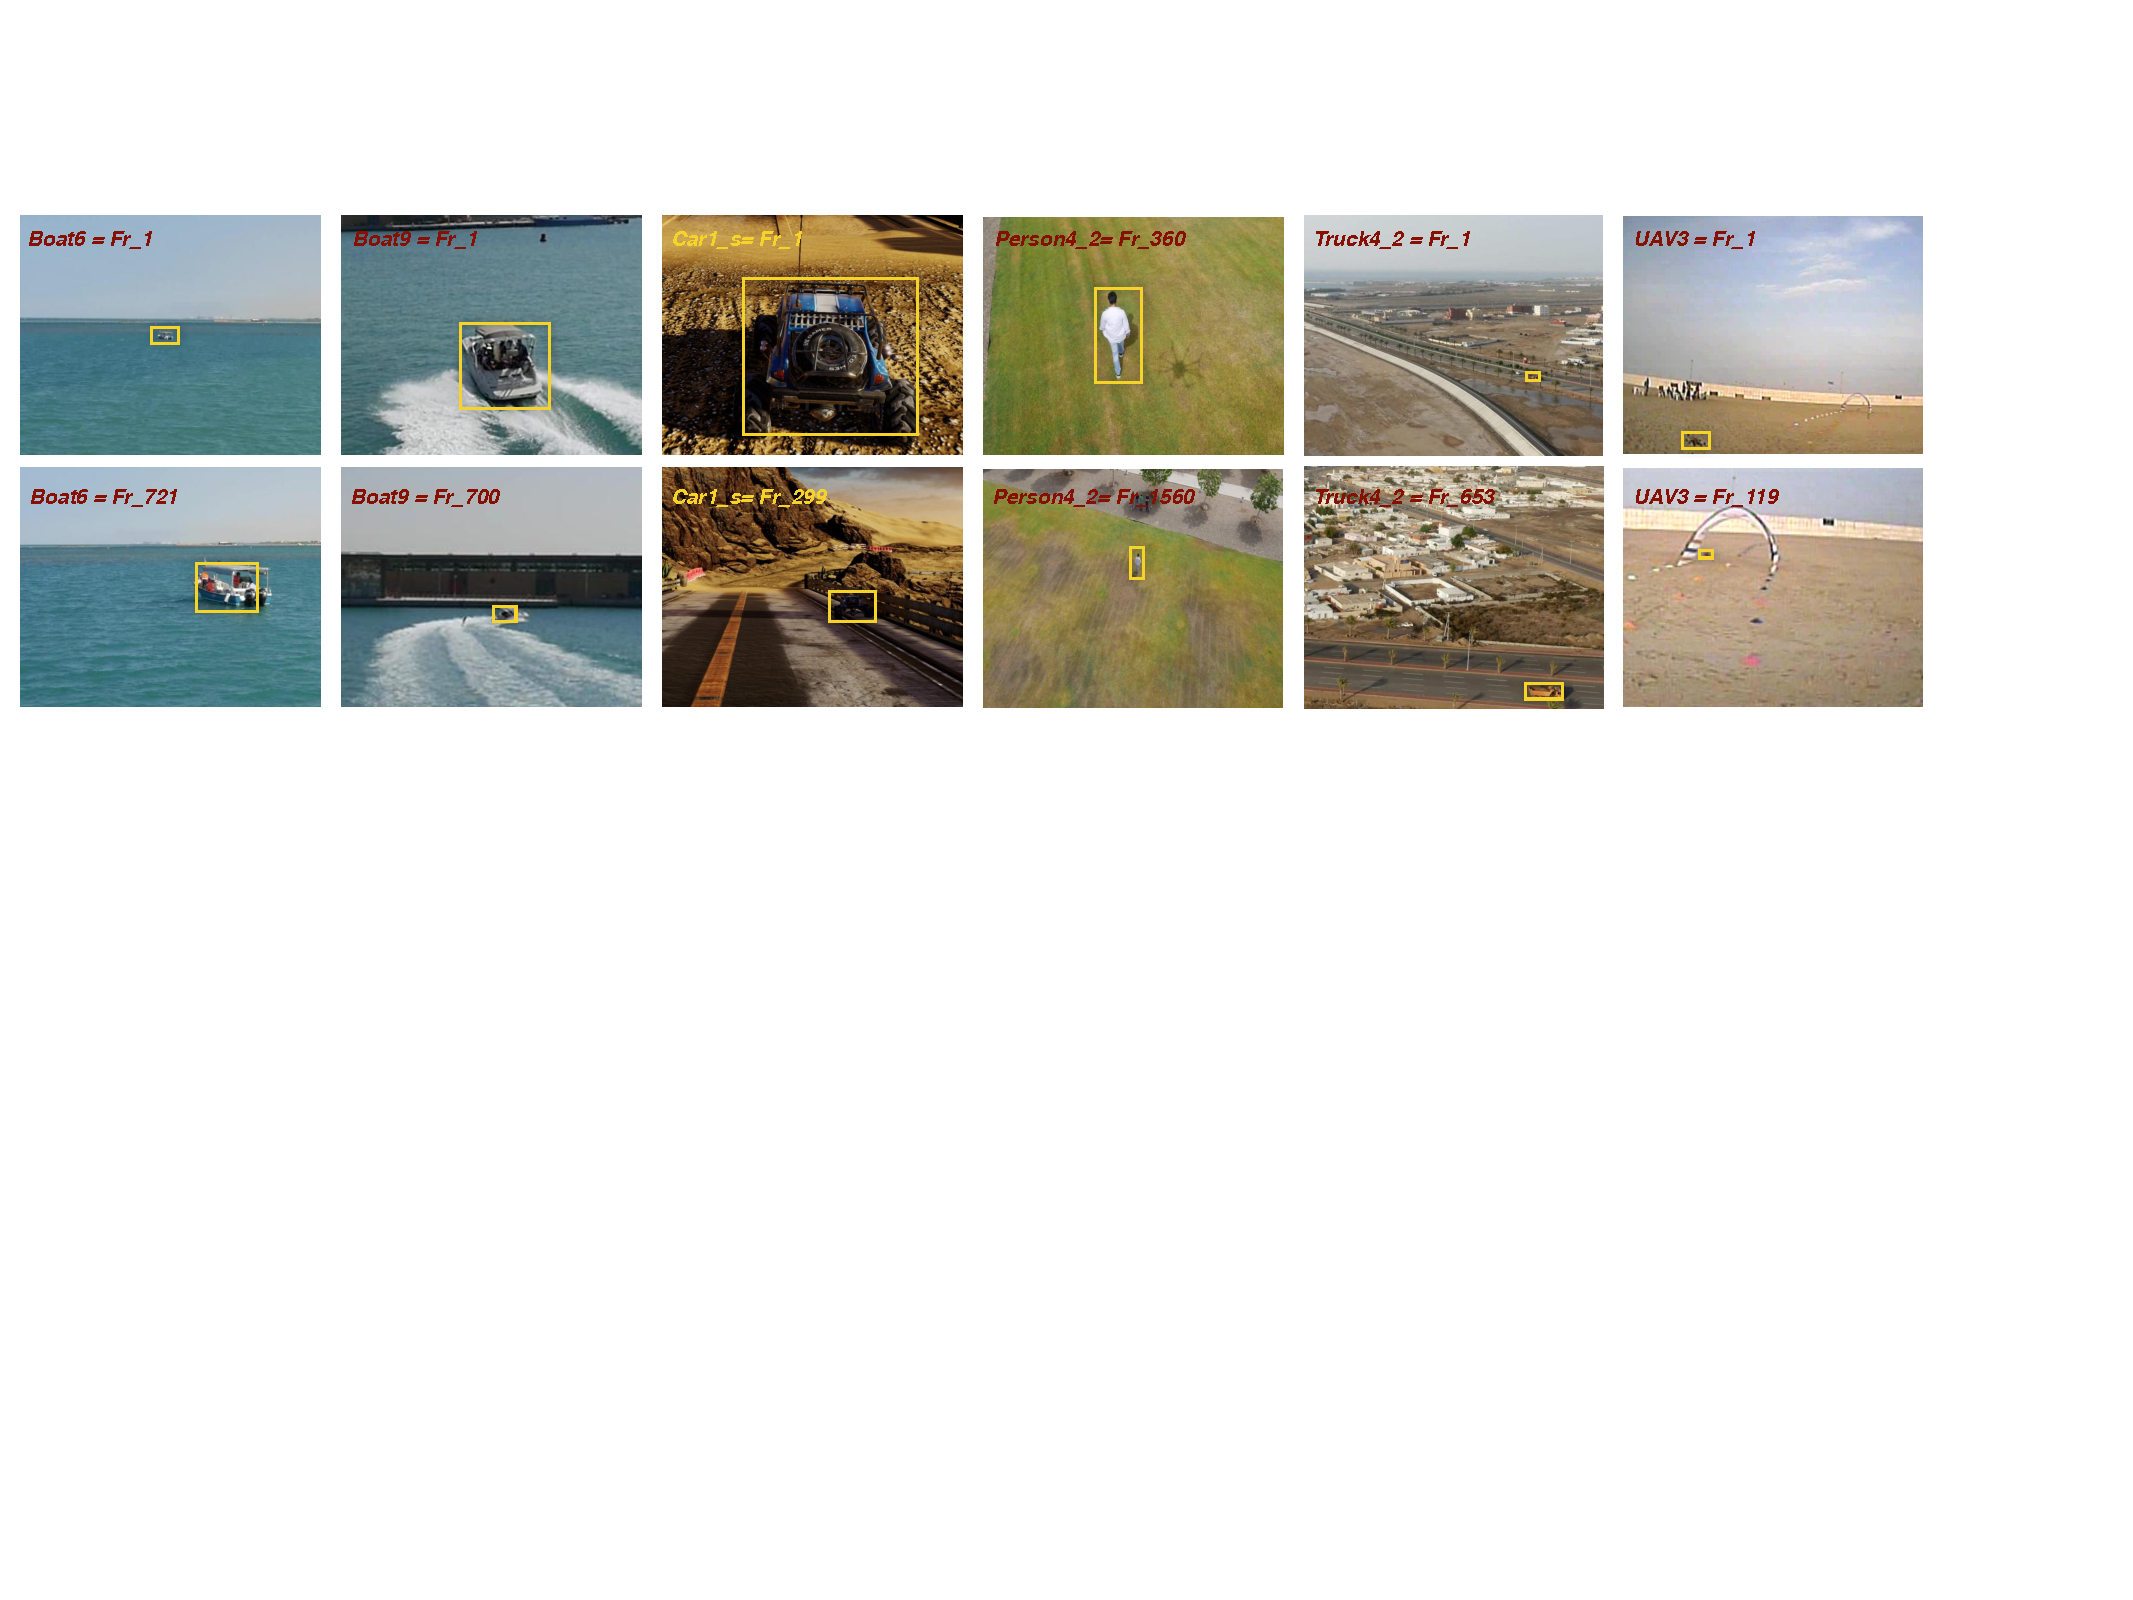
\includegraphics[width=\textwidth]{figures/ResultsIntroduction.pdf}
\caption{Some results of the proposed high-speed ($\geq300$fps) {\it E}nKCF tracker on UAV123 dataset where scale change between the frame in the top row and bottom row is large ($\leq0.5$, or $\geq2$).}
\label{ResultsIntroduction}
\end{figure*}

Another way of handling the scale change for the correlation filter
based approach is to find a correct scale at a location where a target
highly likely appears \cite{zhang2014fast}. In particular, they use
the MOSSE tracker to estimate a target's translation. The scale is
updated in a way where the confidence map is used to determine the
scale change between successive frames. This is because they assume
the scale of a target wouldn't change much over two consecutive
frames. Similarly \cite{ma2015long} used two KCFs to learn the
translation and scale of a target separately. To be more specific, a
KCF is used to learn the translation of the target and its
background. Given this, another KCF is used to learn the target area
to estimate a new scale of the target. However, because of running
more than a KCF on each frame, this method degrades its run-time
performance (i.e., $\leq 50 fps$). Our method is motivated by this
idea -- the idea of deploying multiple KCFs to address the issues of
single target tracking: scale and translation in a highly efficient
manner.  In this paper, we use an ensemble of KCFs in turn, instead of
running them all together on every frame. By doing so, we could still
address the scale change and estimate target's motion efficiently
while increasing run-time performance. In particular, we deploy three
KCF in turn: \textit{target}+\textit{small background} translation
filter ($R_{t}^{S}$), \textit{target-only} scale filter ($R_{s}$) and
\textit{target}+\textit{large background} translation filter
($R_{t}^{L}$). Fig.~\ref{fig:Filters} shows examples of the ROIs
associated with $R_{t}^{S}$, $R_{t}^{L}$, and $R_{s}$.
\begin{comment}
{\it We may not need this.}
The recent progress on development of convolutional neural networks
(CNN) is astonishing as since the AlexNet \cite{krizhevsky12} broke
the record for the ImageNet competition, at every year, new and better
results are reported. Moreover, there have been many attempts to
deploy CNN on the mobile devices
\cite{wu2016quantized,giusti2015}. But the inherent limitation of such
a supervised learning based object tracking is that an either online
\cite{nam2016} or offline \cite{held2016} training tracker has to be
prior to deploy the algorithm.
\end{comment}

\begin{figure}[!t]
\centering
\begin{tabular}{cc}
\bmvaHangBox{\includegraphics[width=12.00cm]{./figures//Workflow_MKCF+PF.pdf}}\\
(a) \\
\bmvaHangBox{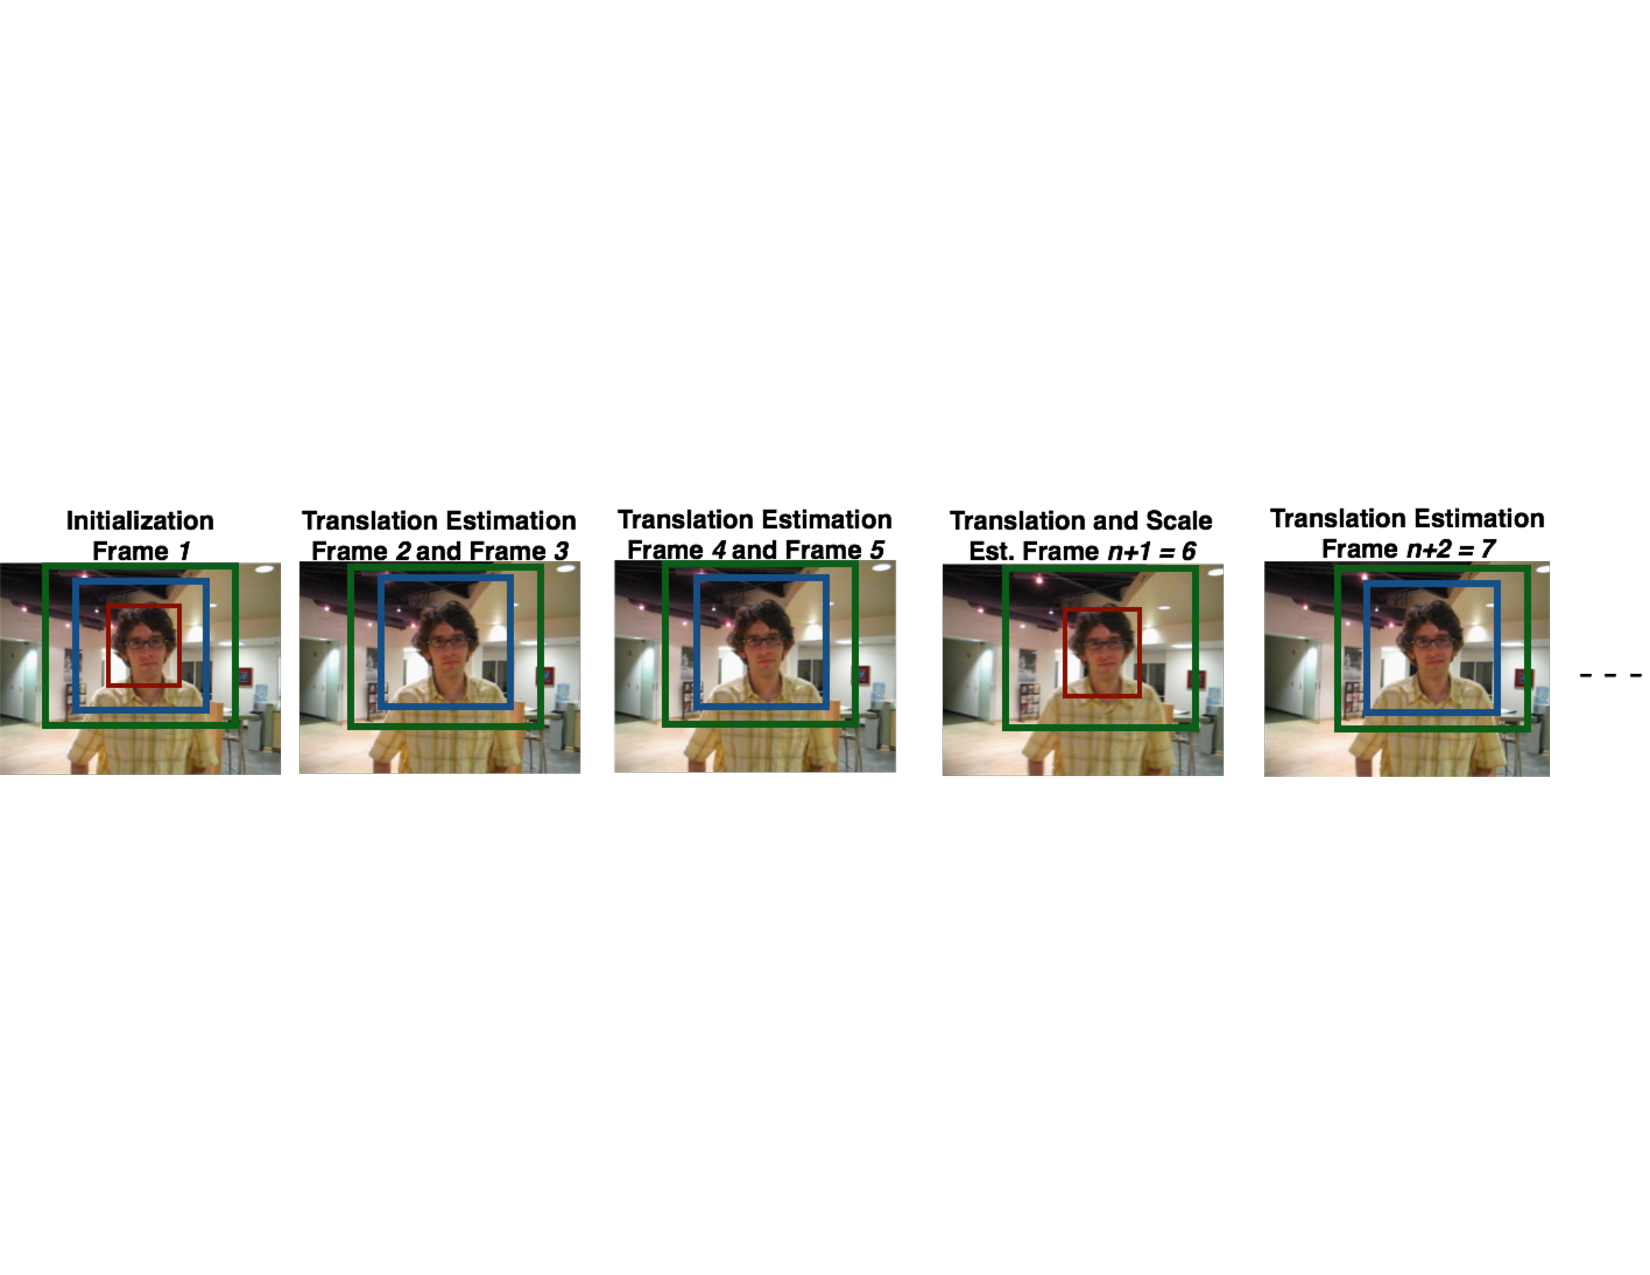
\includegraphics[width=10.0cm]{./figures/Workflow_EnKCF2+PF.pdf}}\\
(b)
\end{tabular}
\caption{The workflow of the proposed $\geq300$fps {\it E}nKCF tracker (a). It is slightly modified to handle extreme ego-motion
and we call it the {\it E}nKCF2 tracker (b) running at $\geq100$fps.}
\label{Workflows}
\end{figure}
The contributions of this study are as follows.
\begin{itemize}
\item \textbf{Novel Single-Target Tracking in a Very High-Speed ($\geq300$ fps) } Our
  algorithm, {\it E}nKCF, deploys an ensemble of KCF in turn to more
  efficiently address the scale variance and the dynamic maneuver of a
  target while preserving run-time performance as high as possible. To
  minimize any potential performance gap from transiting one KCF to
  another, we use a Bayes filter. The workflow of the  {\it E}nKCF can
  be visualized in fig.~\ref{Workflows}. The proposed tracker is tested on UAV123\footnote{\url{https://ivul.kaust.edu.sa/Pages/Dataset-UAV123.aspx}} and OTB100\footnote{\url{http://cvlab.hanyang.ac.kr/tracker_benchmark/benchmark_v10.html}}
  datasets. 

\item \textbf{Slight Modification of the proposed {\it E}nKCF for
  Handling Large Motion} Our second algorithm, {\it E}nKCF2 leverages
  the flexibility of the ensemble of KCFs approach we propose. The
  original {\it E}nKCF is slighlty modified to track in low frame rate
  videos ($10$fps) dominated by large ego-motion. We do not integrate
  the particle filter in {\it E}nKCF2 as we test it on a temporally
  downsampled UAV123 dataset (UAV123$\_$10fps) including sequences
  with large ego-motion on a UAV platform. Particle Filter can be
  deployed in case the camera motion is known. The run-time
  performance decreases to $150$ fps, however, ratio of the video
  frame rate and run-time performance is similar to {\it E}nKCF. The
  proposed framework can be seen in fig.~\ref{Workflows}.
%\begin{figure*}[!t]
%\includegraphics[width=\textwidth]{figures/Workflow_MKCF+PF.pdf}
%\caption{The workflow of the proposed {\it E}nKCF with a particle filter.}
%\label{Workflow_figure_EnKCF}
%\end{figure*}
%\begin{figure*}[!h]
%\centering
%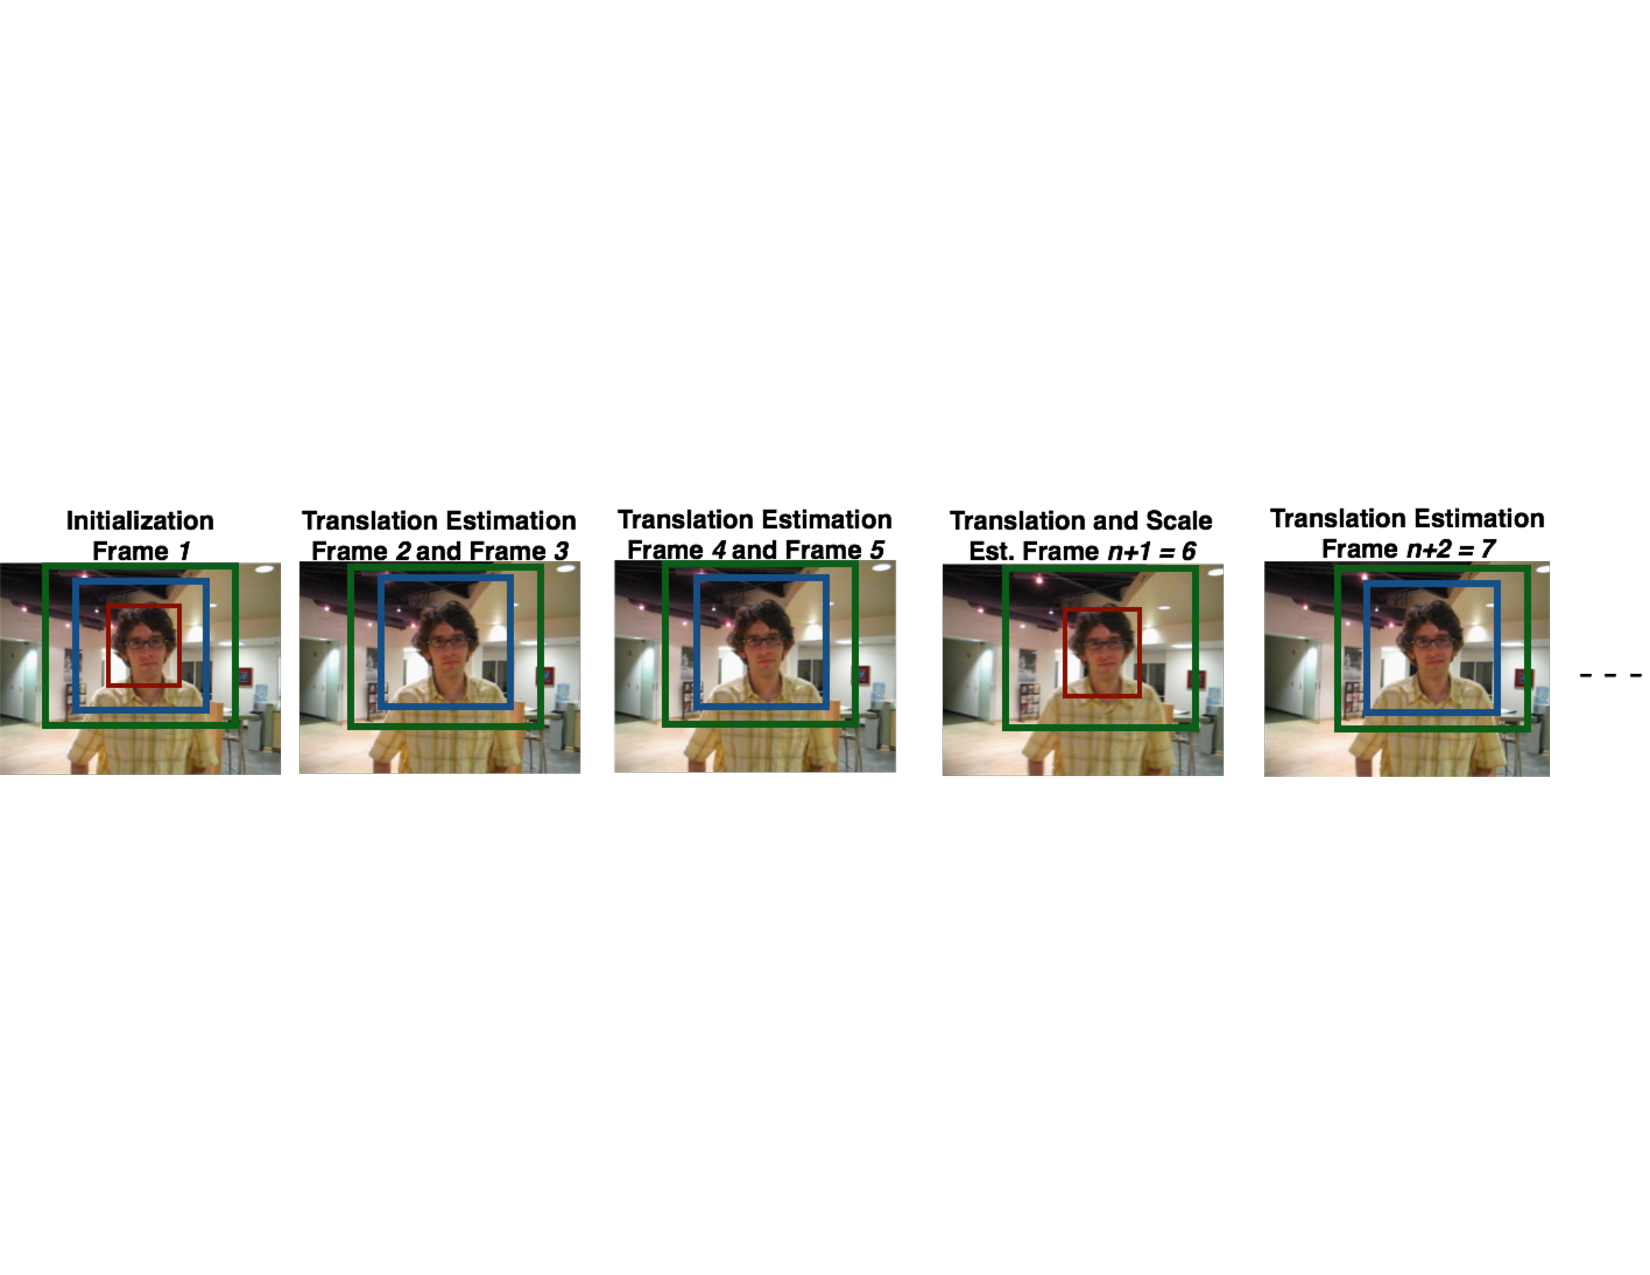
\includegraphics[width=0.75\textwidth]{figures/Workflow_EnKCF2+PF.pdf}
%\caption{The workflow of our {\it E}nKCF2 tracker designed to handle large object motion and ego-motion.}
%\label{Workflow_figure_EnKCF2}
%\end{figure*}

\begin{comment}

\item \textbf{Re-Detection} A target loss is inevitable in object
  tracking. To cope with this, we developed a new target, re-detection
  that reliably detects when to lose the target and effectively
  re-detect the lost target. {\it How we can show how good our
    re-detection method is?}

\item We build a highly efficient ($\geq300$ fps) scale adaptive
  multiple kernelized correlation filter based tracker that
  outperforms the original KCF implementation with fixed scale
  framework both in terms of accuracy and performance. The studies
  following the KCF improved the fixed scale framework by running
  detection on a number of candidate ROIs to figure out the new scale
  of the object after estimating the translation of the object. This
  approach adds additional complexity to the original KCF
  implementation and drags down the run-time performance from $300$
  fps to less than $100$ fps.

\item We propose a target re-detection module that can minimize the
  target loss due to the scale filter that learns the object model
  using only-object area. Also, the target re-detection step is
  required to handle severe occlusions, pose variations, illumination
  changes and fast motion.

\item Since our visual tracker mostly focuses on tracking objects from
  aerial moving platforms, we design a new robust target-to-camera
  distance estimation method. This way, a safe distance between the
  target and the camera-platform can be preserved.
\end{comment}

\end{itemize}

%---------------------------------------------------------------------- 
\section{{\it E}nKCF: Ensemble of Kernelized Correlation Filters}
%---------------------------------------------------------------------- 
In this paper, we extend the KCF in that multiple KCFs are deployed,
in turn, to address a target's scale change and dynamic maneuvers
while preserving the overall execution time very fast, i.e., $\ge$ 300
fps. The efficient nature of KCF computation results in a
small-footprint, executable. Such a fast execution will facilitate to
deploy the proposed algorithm on any embedded systems.

The proposed algorithm, {\it E}nKCF, deploys three KCFs in turn: The
first filter, $R_{t}^{S}$, focuses on learning the target area and its
background, \textit{target}+\textit{small background} for addressing a
marginal translation by a target, the second filter, $R_{s}$, focuses
entirely on learning the target's scale, \textit{target-only}, and the
last filter, $R_{t}^{L}$, focuses on the target area and its
background twice bigger than that of the first filter, $R_{t}^{S}$,
\textit{target}+\textit{large background}. We set up {\it E}nKCF in
this way because we believe a correlation filter for learning a
target's translation should include its background to better
discriminate the target from its background and another correlation
filter is prepared to focus on the target itself to estimate the right
size or scale of the target. Fig.~\ref{fig:Filters} shows examples
of the region of interest (ROI) covered by each of three filters. We
believe that a filter for learning a target's translation should
include its background. In addition, making the ROI for the scale
filter, $R_{s}$, tighter reduces the size of the template for the
elementwise multiplication, resulting in a scale estimation in a
higher speed.
\begin{figure}[!h]
\centering
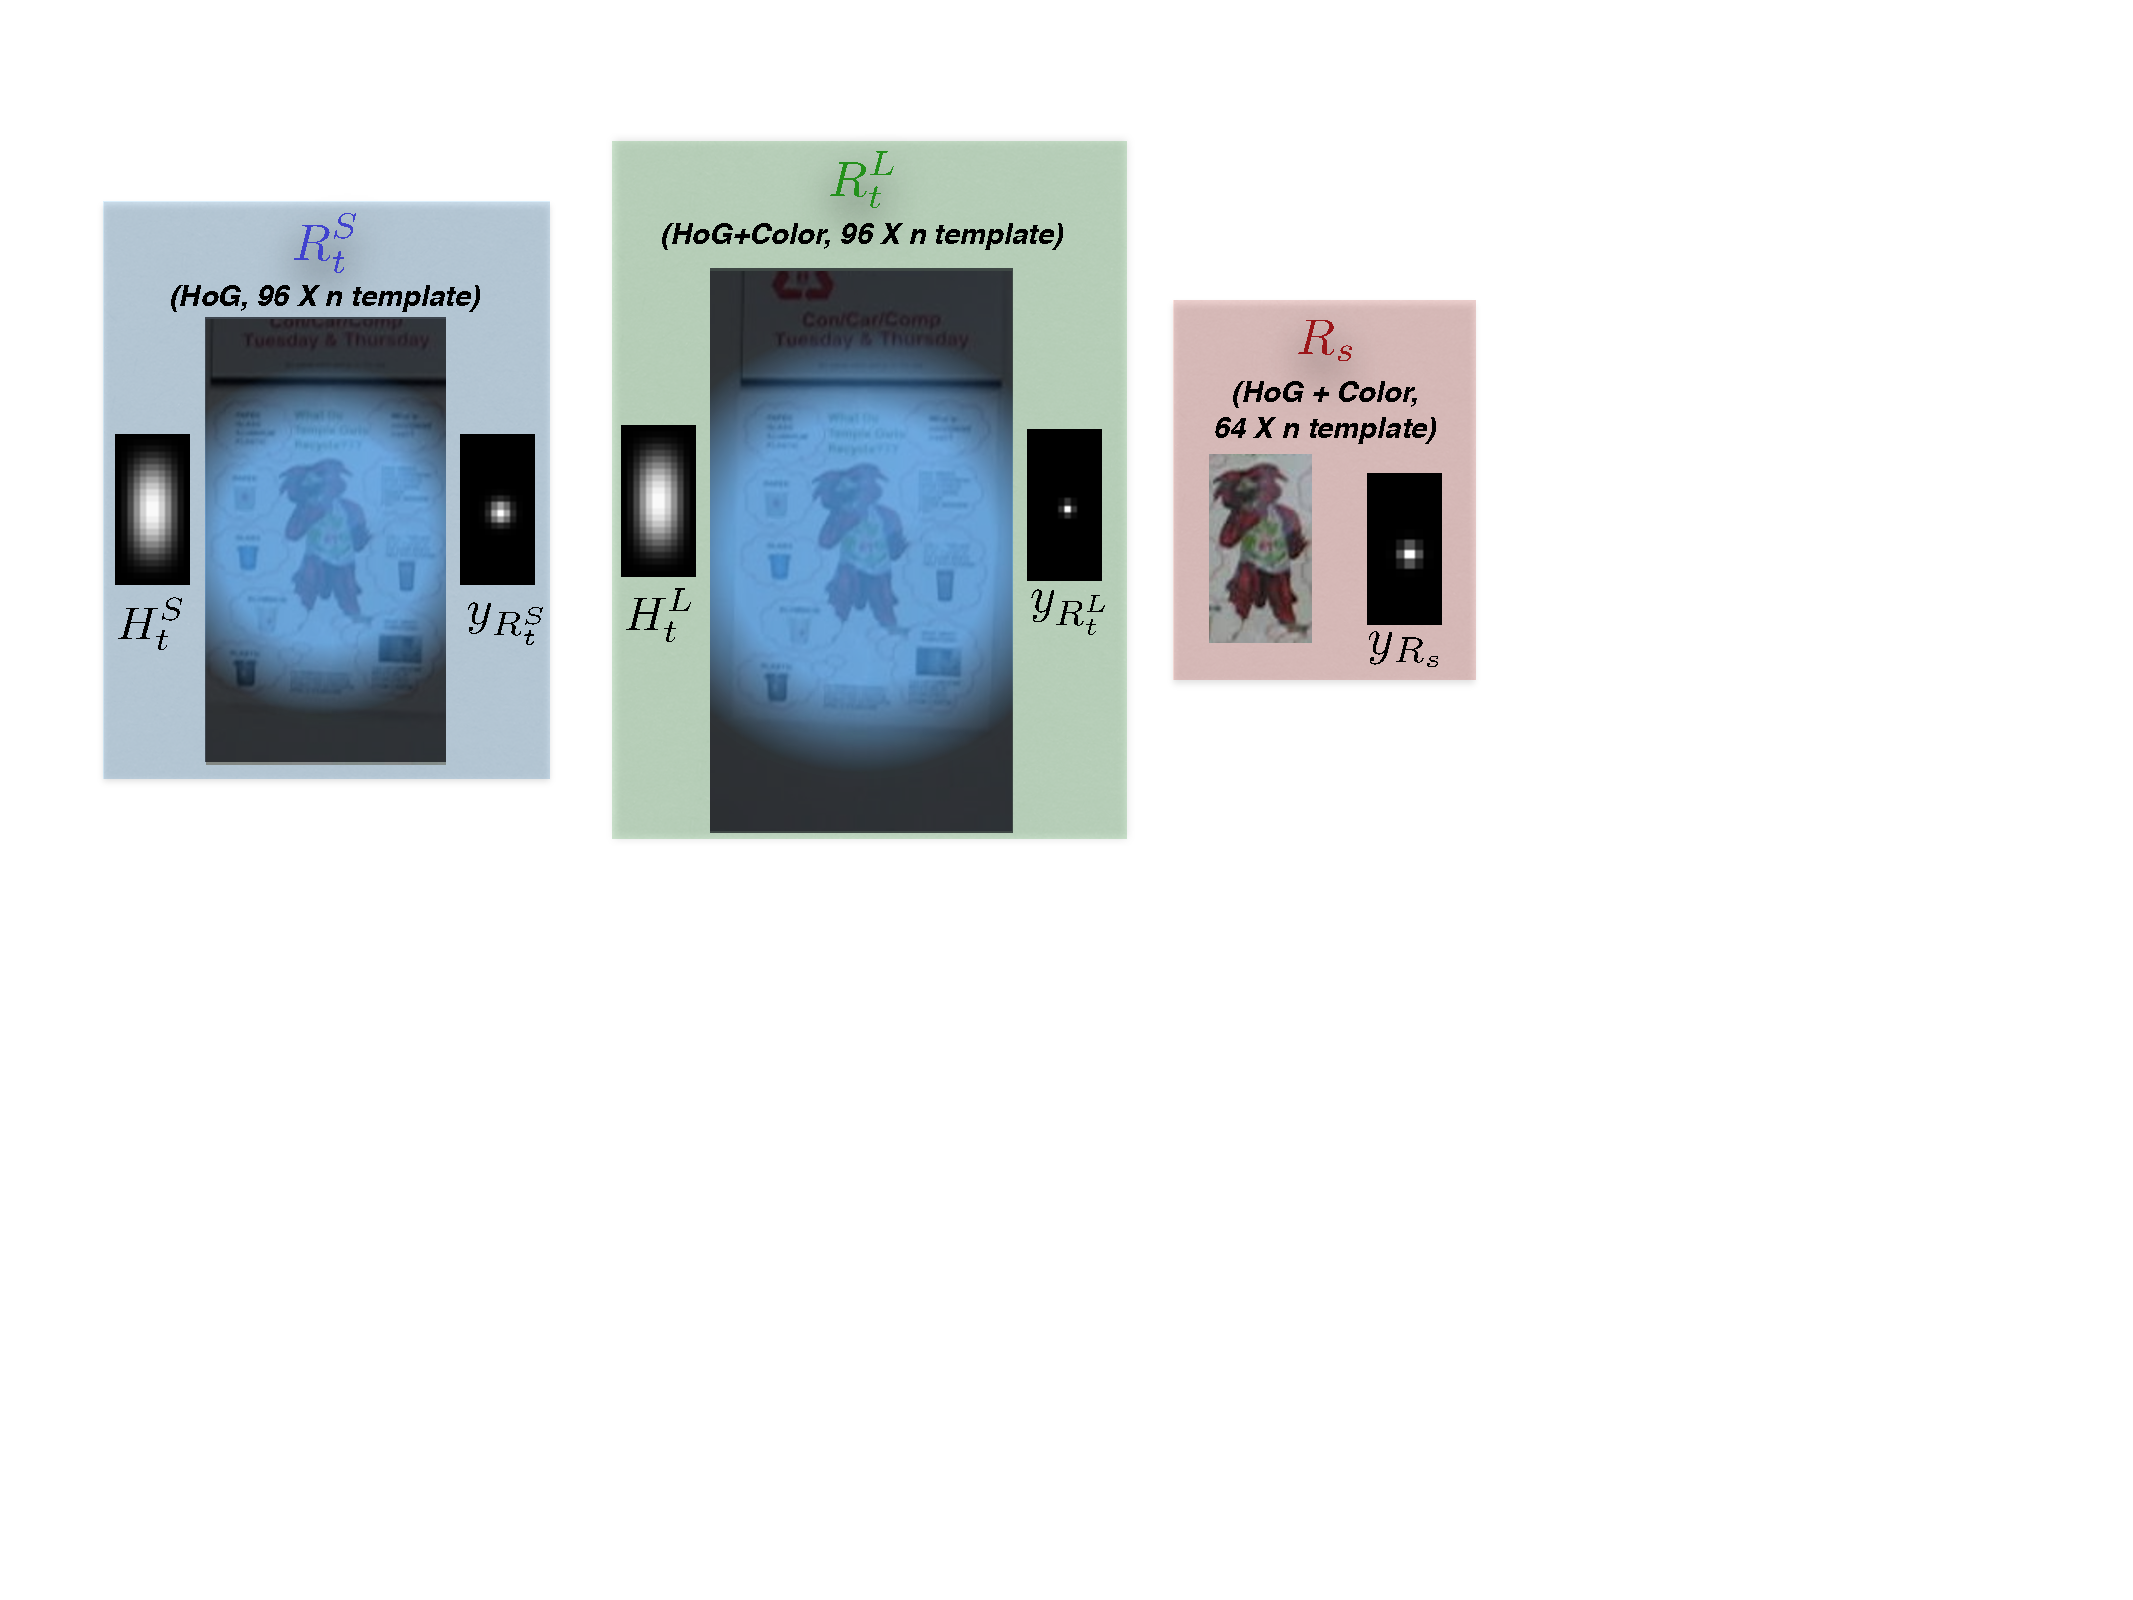
\includegraphics[width=0.5\textwidth]{figures/Filters_Details.pdf}
\caption{The three filters denoted as \textit{target+small background} translation filter,
  \textit{target-only} scale filter and \textit{target+large background} translation filters are
  shown. Also, the hanning window and desired Gaussian response for
  each filter is displayed.}
\label{fig:Filters}
\end{figure}

After Henriques and his colleagues' presented impressive tracking 
results of KCF \cite{henriques2015high} on
VOT15\footnote{\url{http://www.votchallenge.net/vot2015/}} challenge,
many variation of KCF were investigated. In particular,
\cite{ma2015long} and \cite{danelljan2014accurate} used a scale filter
to learn the target area only whereas \cite{li2014scale,
  bibi2015multi, tang2015multi} used a correlation filter learned on
the target area and its surrounding background in different size to
learn the optimal scale of the target. Our approach is particularly
similar to that of \cite{ma2015long} in that more than one KCF is used
to address the challenges of single target tracking. But ours is
different from that of \cite{ma2015long} in that we do not use those
multiple KCFs together at every frame, but alternatively at every
three frame. The way our algorithm is alternating multiple KCFs in
different goals intuitively makes sense in that the appearance of
consecutive images does not change drastically. Although it varies
based on the scene, learning a correlation filter a frame would not be
much different from the one learned using the image few or $k$ frames
later. By alternating three KCFs in turn, our algorithm runs as fast
as or faster than the original KCF. From our experiments, we
empirically found that five is the optimal for $k$ in terms of
precision and success rates. We'll detail this at the experimental
section later.

\begin{figure}[!h]
\centering
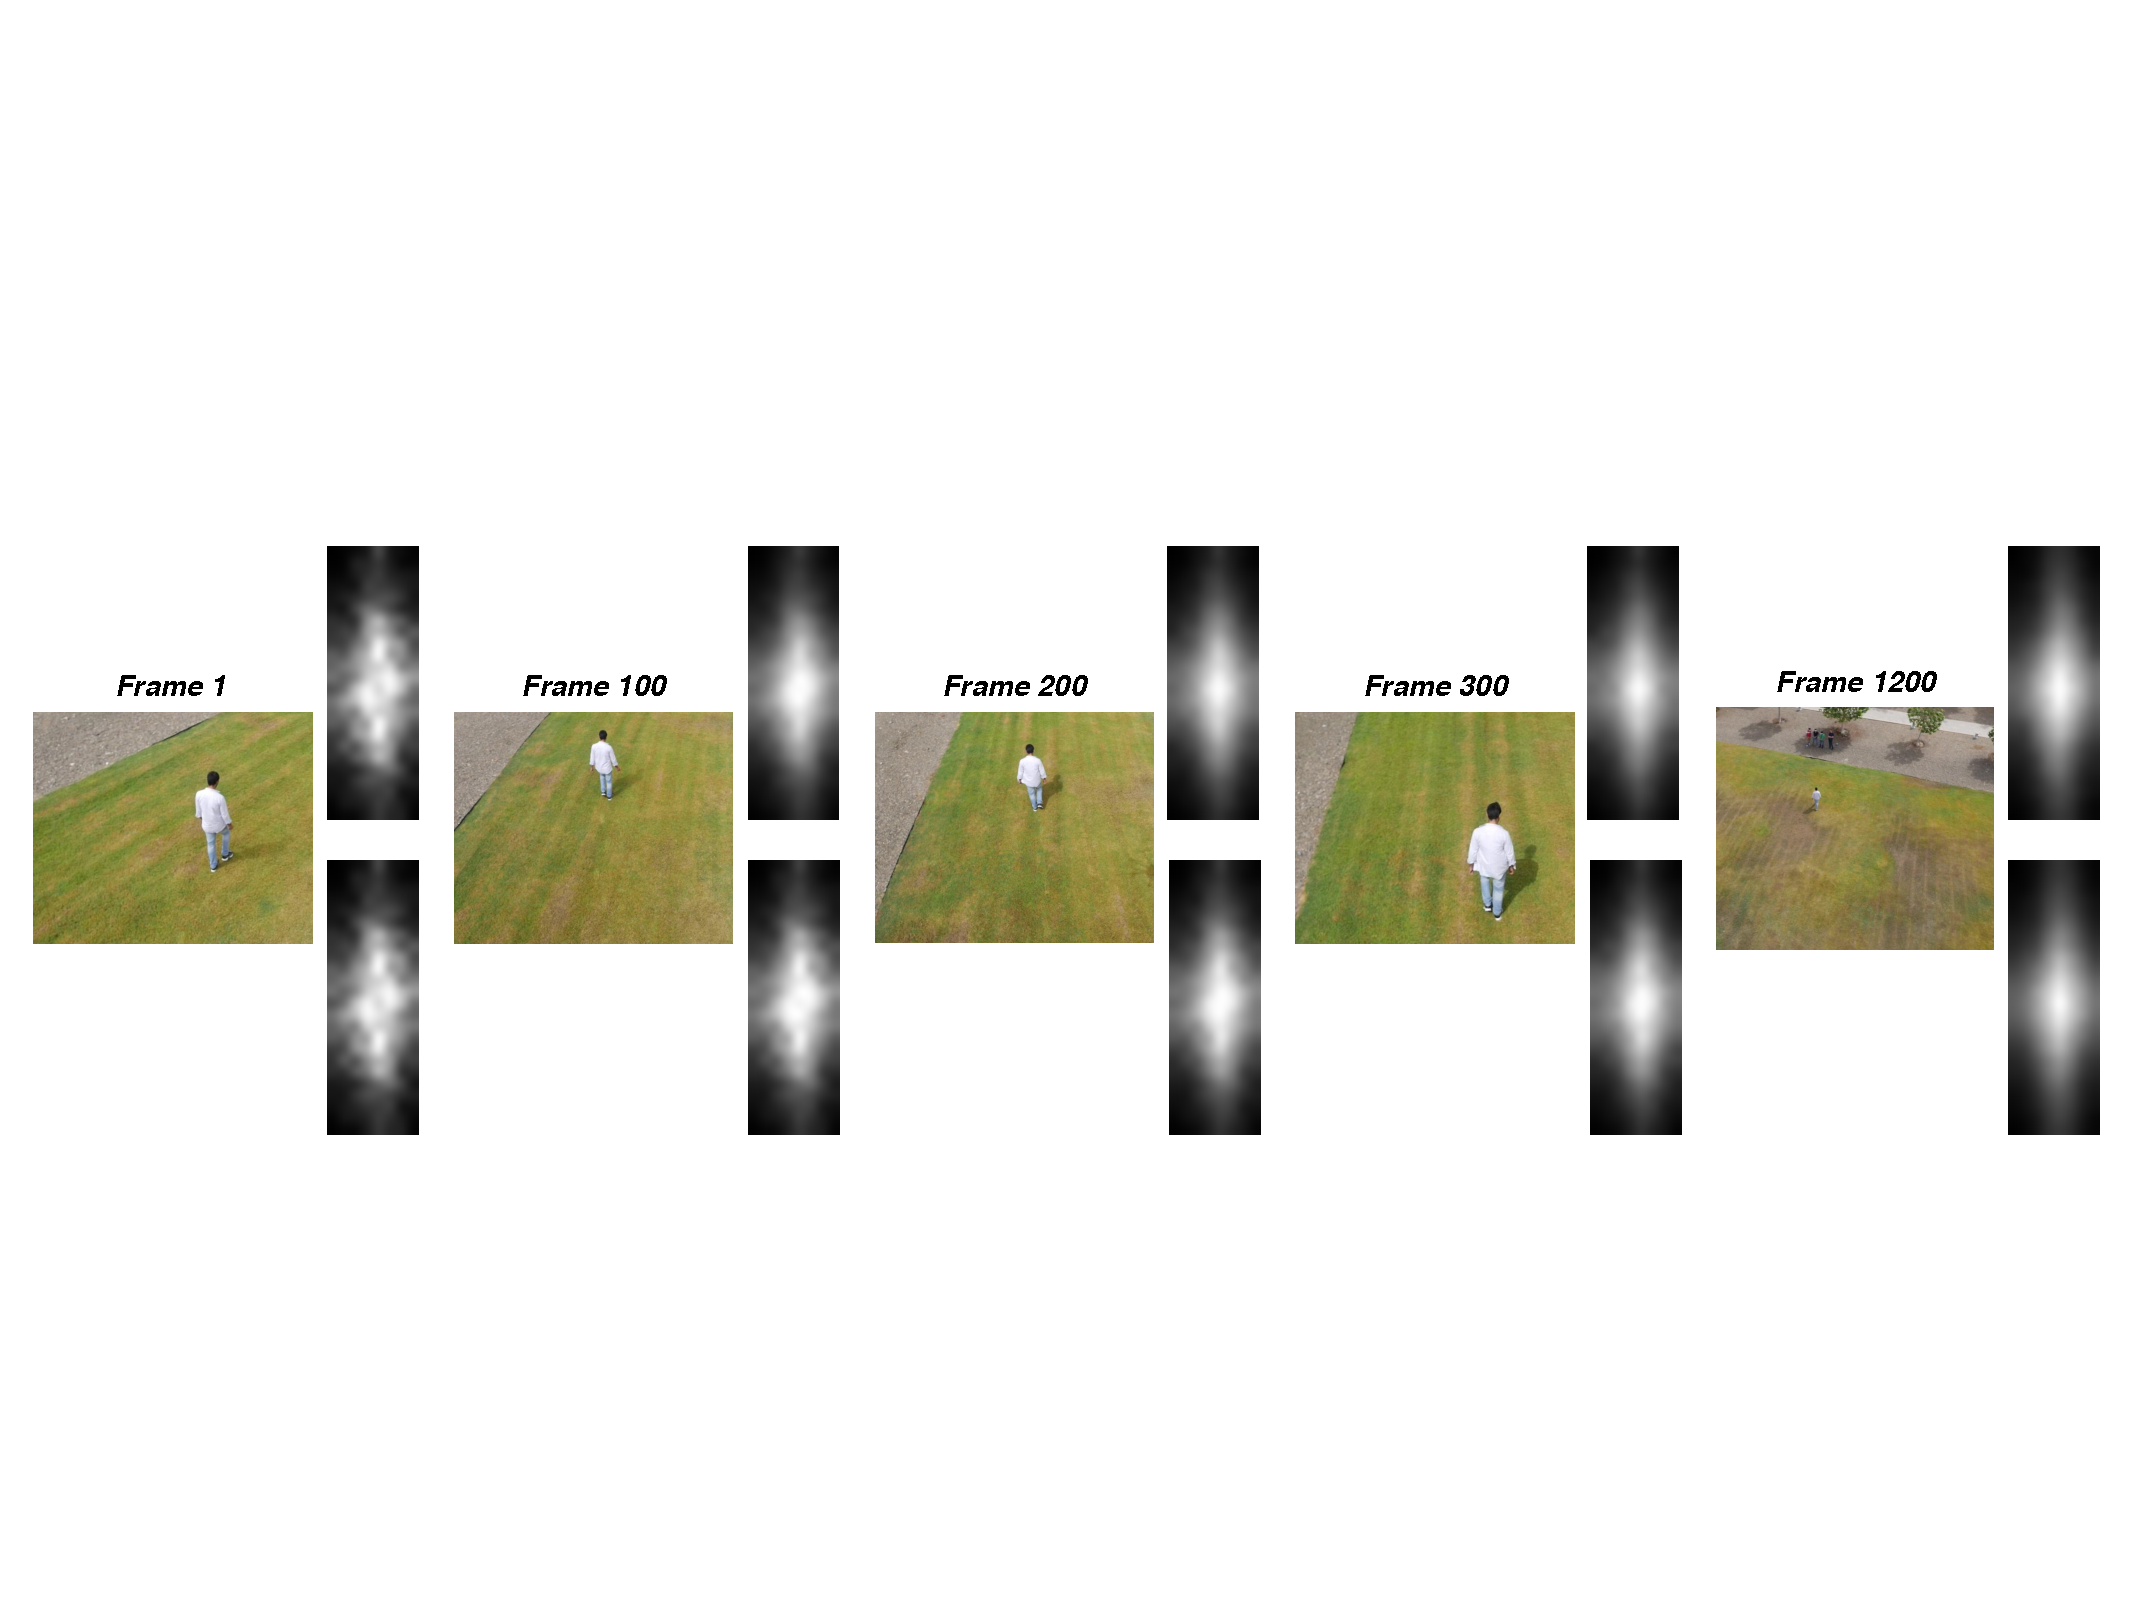
\includegraphics[width=0.75\textwidth]{figures/LearnedFilterComparison.pdf}
\caption{The video frame and the learned scale correlation filters are shown next to it. 
The models in the top row correspond to the scale filter trained every frame whereas the bottom row shows the scale filter updated every $5$ frames. 
Filters updated every five frame and every frame display very large correlation.}
\label{fig:Filters_Comparison}
\end{figure}

The order of running these three KCFs is important as each of these
filters aims at addressing different chanllenges while perserving
run-time performance as fast as possible. The \textit{target+large
  background} translation filter, $R_{t}^{L}$, is intended to run
right after the scale filter, $R_s$, runs which is applied at every
$k=5$ frames. We run these two filters this way because we want to
minimize any drifts that are likely to happen running only $R_{s}$. In
addition, the filter, $R_{t}^{S}$, is applied to every other frames
before $R_{S}$ and right after two consecutive frames running
$R_{t}^{L}$. By doing so, we can integrate more discriminative shape
features that can not be fully learned by $R_{t}^{L}$ as it contains
contribution of large background in the learned model. The filter,
$R_{t}^{L}$, uses shape and color information together to recover from
any potential drifts -- drifts could happen only looking the target's
scale by the filter, $R_{s}$.

In summary, the scale filter, $R_{s}$, is designed to directly handle
the scale change of a target and provides $R_{t}^{L}$ and $R_{t}^{S}$
with more focused ROIs about the target's translation. A translation
filter, $R_{t}^{L}$, is intended to look at a larger search area to
estimate the target's translation and recover from any potential
drifts. Another translation filter, $R_{t}^{S}$, on the other hand, is
designed to addresses the drawback of $R_{t}^{L}$ that it may learn
noisy shape features due to its large search area. Figure
\ref{Workflows} illustrates the workflow of the proposed
algorithm and alg.\ref{alg:MKCF} shows the pseudo-code of {\it
  E}nKCF. We do not have a seperate pseudeo-code for {\it E}nKCF2 as there are only two differences between 
  {\it E}nKCF and {\it E}nKCF2. First, the {\it E}nKCF2 runs $R_{t}^{L}$ every frame
to better tackle large ego-motion at low video frame rates. Second, we remove the particle filter in the {\it E}nKCF2 
tracker due to large ego-motion. In the following section, we will briefly mention the theory
behind the KCF.

\begin{algorithm}
	\caption{The {\it E}nKCF Tracking Algorithm.}\label{alg:MKCF}
	\begin{algorithmic}[1]
	\State \textbf{Input} : Initial bounding box $x_{0}$, frame counter $fc$, scale filter frequency $n = 5$,
	\State \textbf{Output} : 
				\If{$fc\:\%\:n=0$} \Comment{Condition 1}
						\State Estimated Target State $x_{t} = (x_{t},y_{t},s_{t})$,
						Scale filter (\textit{target-only}) model $R_{s}$.
			     \EndIf
				\If{$fc\:\%\:n=1\:\:or\:\:fc\:\%\:n=2$}\Comment{Condition 2}
						\State Estimated Target State $x_{t} = (x_{t},y_{t},s_{t_1})$,
						Large Area Translation Filter model $R_{t}^{L}$.
				\EndIf
				\If{$fc\:\%\:n=3\:\:or\:\:fc\:\%\:n=4$}\Comment{Condition 3}
						\State Estimated Target State $x_{t} = (x_{t},y_{t},s_{t})$,
						Small Area Translation Filter model $R_{t}^{S}$.
				\EndIf
	\Procedure{track}{$x_{t-1},y_{t-1},s_{t-1}$} 
				\State // Translation Estimation
				\State Transit Particle Filter to the frame $t$ and compute the mean of prior pdf $x_{t} = (x_{t},y_{t},s_{t-1})$;
				\State // Translation Estimation
				\State Crop the ROI for the $R_{t}^{L}$, or $R_{t}^{S}$ given $x_{t}$
				and estimate translation ($x_{t}$,$y_{t}$) using $R_{t}^{L}$ (Condition 2) or $R_{t}^{S}$ (Condition 3),
				\State Skip translation estimation for $R_{s}$ (Condition 1);
				\State // Scale Estimation
			    \State Crop the ROI for the $R_{s}$ and estimate scale, $s_{t}$, using $R_{s}$ (Condition 1), 
				\State Scale pool for $R_{s}$ : $\lbrace1.05,1.0,1/1.05\rbrace$;
		        \State Skip it for $R_{t}^{L}$ and $R_{t}^{S}$ (Condition 1, and 2),
				\State // Update Translation
				\State Perform Importance Re-sampling (if necessary) for Particle Filter and compute the mean of posterior pdf $x_{t} = (x_{t},y_{t},s_{t})$;
			    \State // Model Update
				\If{$PSR(y_{R_{s}}) \geq T_{R_{s}}$}
				\State Update $R_{s}$ (Condition 1);
				\EndIf							 
				\If{$PSR(y_{R_{t}^{L}}) \geq T_{R_{t}^{L}}$} 
				\State Update $R_{t}^{L}$ (Condition 2);
				\EndIf	
			     \If{$PSR(y_{R_{t}^{S}}) \geq T_{R_{t}^{S}}$}
				\State Update $R_{t}^{S}$ (Condition 3);
			     \EndIf		
	\EndProcedure	
	\end{algorithmic}
\end{algorithm}

\begin{comment}
{\it Burak: The KCF section doesn't fit the section before and
  after. In addition, it's still too long.}
  
{\it YoungWoo : What do you mean by this? Should we move it up before the EnKCF introduction? or Should we include more EnKCF-related text in it? I trimmed it further. I wanted to keep some equations because they include hyper-paramaters that is important for EnKCF.}
\end{comment}

\subsection{Kernelized Correlation Filter} \label{sec:kcf}
The Kernelized Correlation Filter tracker has recently been
increasingly popular due to its operation at hundreds of frames per
second with state-of-the-art tracking capabilities even in challenging
cases. Its computational efficiency arises from its use of the
discrete fourier transform of the circulant matrix and frequency
domain element-wise operations known as hadamard product and
division. The first example of frequency domain trackers is the MOSSE
tracker running at $700$fps \cite{bolme2010visual}. It minimizes the
ridge regression function in the frequency domain using a single
template and intensity features. The KCF tracker, on the other hand,
minimizes the regularized ridge regression function shown below.
\begin{equation}
E(h) = \frac{1}{2}||y-\sum_{c=1}^{C}h_{c}*x_{c}||^{2} + \frac{\lambda}{2}\sum_{c=1}^{C}||h_{c}||^{2}
\label{eq:Closedform_RidgeReg}
\end{equation}
where $y$ represents the desired continous response whereas $h$ and
$x_{c}$ represents the learned correlation filter and training
template for the given channel. The $c$ parameter included in
\cite{henriques2015high,galoogahi2013multi} makes it possible to
integrate multi-channel features such as HoG and colour into the ridge
regression function. The closed-form solution for the
eq.~\ref{eq:Closedform_RidgeReg} can be obtained by setting the
derivative of $E$ w.r.t $w$ to $0$. The primal solution in the
frequency domain is formulated as
%\begin{equation}
%w = (X^{T}X+\lambda)^{-1}y
%\label{eq:SpatialSolution}
%\end{equation}
\begin{equation}
w = (X^{H}X+\lambda I)^{-1}X^{T}y
\label{eq:FourierSolution}
\end{equation}
where $X^{H}$ and $\lambda$represent the complex-conjugate of training
samples and regularization term. More documentation on the spatial and
fourier domain solutions can be found in \cite{henriques2015high}. The
MOSSE tracker uses one training sample centred at estimated position
of the target. This framework does not include enough background
information into the learned model,$w$. The application of the
circulant matrix theorem into the eq.~\ref{eq:Closedform_RidgeReg}
makes it possible to include many background patches at a similar
computational complexity. A circulant matrix includes the circularly
shifted patches of the positive training sample $x$ by a cylic shift
operator.

%By applying shifting operation to the base sample, we can generate the circulant
%matrix as
%\begin{equation}
%C = Px.
%\label{eq:CirculantMatrixGeneration}
%\end{equation}
%The circulant matrix of a base sample $x$ can be interpreted as the
%rows of a training matrix $X$ where each row represents features of a
%training sample. Mathematically, this can be written as
%\begin{equation}
%X = C(x)
%\label{eq:CIrculantMatrixTrainingData}
%\end{equation}

In this form, the equation \ref{eq:FourierSolution} could prohibit us
from implementing a high speed object tracking as we need to perform
large number of element-wise division and multiplication
operations. However, we know from \cite{gray2006toeplitz} that all
circulant matrices are represented diagonally by the Fourier Transform
regardless of the base sample $x$.
%\begin{equation}
%X = Fdiag(\hat{x})F^{H},
%\label{eq:CirculantMatrixDFT}
%\end{equation}
%where $F$ denotes a constant Fourier Transform matrix and $x$ is the
%Discrete Fourier Transform of the base sample $x$. 
%To simplify the
%cost function formulation in eq.~\ref{eq:FourierSolution} we multiply
%$X$ in eq.~\ref{eq:CirculantMatrixDFT} with $X^{H}$ yielding
%\begin{equation}
%X^{H}X = Fdiag(\hat{x}^{*}\odot \hat{x})F^{H}.
%\label{eq:SimplificationX} 
%\end{equation}
Then, the optimized solution vector in the Fourier domain $\hat{w}$ is formulated as
\begin{equation}
\hat{w} = \hat{x}^{*}*\hat{y}(\hat{x}^{*}*\hat{x}+\lambda)^{-1}.
\label{eq:DiagonalizedPrimalSolution}
\end{equation}
To further improve the robustness to geometric and photographic variations, one can exploit non-linear
regression function in the Correlation Filter framework \cite{henriques2015high}. 
%\begin{equation}
%\alpha = y(K+\lambda I)^{-1}
%\end{equation}
%where $K$ and $\alpha$ represent the kernel matrix and corresponding
%dual space solution. 
%\cite{henriques2015high} states that kernel
%matrices is circulant for datasets of circular cylic satisfying the
%following theorem.
%\begin{equation}
%k(x,x^{'}) = k(Mx,Mx^{'}),
%\label{eq:KernelCirculantTheorem}
%\end{equation}
%where $M$ represents the permutation matrix. Some kernels satisfying
%the eq.~\ref{eq:KernelCirculantTheorem} are \textit{Gaussian},
%\textit{Polynomial}, \textit{Intersection} and \textit{Hellinger}
%kernels. 
Similar to the diagonalization in the linear ridge regression
solution in eq.~\ref{eq:DiagonalizedPrimalSolution}, the kernelized
ridge regression can be made diagonal using the same circulant matrix
theorem.  The diagonalized Fourier domain dual form solution can be
expressed as
\begin{equation}
\hat{\alpha} = \hat{y}(\hat{k}^{xx}+\lambda)^{-1}
\label{eq:FourierDualDomainSolution}
\end{equation}
where $\hat{k}^{xx}$ represents the first row of the Kernel matrix $K$
known as \textit{gram matrix}. In this study, we will only focus on
application of the Gaussian Kernel to the Correlation Filters. We
refer the readers to \cite{henriques2015high} for the detailed
documentation of the application of other kernels to the Correlation
Filters. The Gaussian kernelization is
expressed as
\begin{equation}
k^{xx^{'}} = exp(-\dfrac{1}{\alpha^{2}}(||x||^{2}+||x^{'}||^{2}-2F^{-1}(\sum^{C}_{c}\hat{x}_{c}^{*}\odot \hat{x}_{c}^{'}))).
\label{eq:GaussianCorrelationSingleChannel}
\end{equation}
%\begin{equation}
%k^{xx^{'}} = exp(-\dfrac{1}{\alpha^{2}}(||x||^{2}+||x^{'}||^{2}-2F^{-1}(\hat{x}^{*}\odot \hat{x}^{'})))
%\label{eq:GaussianCorrelationSingleChannel}
%\end{equation}
The first correlation filter based trackers used grayscale feature ($C=1$) to
learn the solution vector $w$, however, multi-channel features
such as HoG and Color were later exploited to improve tracking
accuracy \cite{henriques2015high,galoogahi2013multi,tang2015multi,ma2015long,bibi2015multi}. The
multi-channel feature integration into the Gaussian Kernelization
function in eq.~\ref{eq:GaussianCorrelationSingleChannel} is achieved
in a very straight-forward way by summing the correlation result over the channels.

Training shown in eq.~\ref{eq:FourierDualDomainSolution}
gives us $\hat{a}$ learned in time step $t$. We can accumulate
$\hat{a}$ over time to integrate more temporal information. This can
be expressed as
\begin{equation}
\hat{a}_{t} = (1-\beta)\hat{a}_{t-1} + \beta\hat{a}_{t}. 
\end{equation}

Finally, detection step in multi-channel KCF framework is performed as
\begin{equation}
r(z) = F^{-1}(\hat{k}^{xz} \odot \hat{\alpha})
\end{equation}
where $r$ denotes the correlation response at all cylic shifts of the
first row of the kernel matrix $K$. The peak point of the response
function gives us the estimated translation of the object from time
step $t$-$1$ to $t$.

\subsection{Particle Filter for Smoothing Transition of KCFs} \label{sc:PF}
As explained earlier, the {\it E}nKCF upates a target's translation at
every other $k$ frames, particularly for estimating the target's
scale. Although the strategy of updating every other $k$th frames will
result in an optimal run-time performance, this may lead any potential
drifts at the later frames. To prevent such potential mishaps from
happening, we developed a Bayes filter that incorporates a target's
motion to smooth any outputs from the {\it E}nKCF. In particular, we
use a particle filter to estimate the target's image coordinate based
on the {\it E}nKCF's outputs. A particle filter is a sequential Monte
Carlo method that uses a finite number of particles or samples to
estimate the posterior probability density of a state of the system
\cite{thrun2005probabilistic}. In this study, the state represents a
target's pixel coordinates and its motion. In particular, the state of
the particle filter, $X_t$, is represented by $\lbrace x, y, v_{x},
v_{y} \rbrace$, where $x$ and $y$ are the pixel coordinates of the
target's centroid, $v_x$ and $v_y$ are the estimated velocity along
the $x$-axis and $y$-axis. The particle filter predicts, using a
constant velocity motion model, a target's state by generating a
predefined number of particles. And then the particle filter uses the
confidence maps of {\it E}nKCF as observation to update the state. The
weight of a particle is computed as:
\begin{equation}
w_{p_{t}}(x_{t},y_{t}) = \sum_{i=1}^{N}\sum_{j=1}^{N} y_{R}(x_{t}-i,y_{t}-j)
\end{equation}
where $w_{p}$ denotes the weight of the particle $p$ at time $t$ and
$N$ denotes the size of the window as that of a confidence
map. Alternatively one can also use the euclidean distance of
particles to the location of maximum response of the confidence
map. This alternative, however, would result in drifts. 

We chooses some particles based on their importance to estimate the
target's next state, i.e., its pixel coordinates as $\hat{X}_{t} =
\sum_{p=1}^{P}w_{p_{t}} X_{t}.$ Note that, unlike a typical operation
of a particle filter, we skip the importance re-sampling step when the
scale filter, $R_{s}$, estimates the target's scale change. This is
because we observe the confidence map from the scale filter, $R_s$ is
sometime noisy. In addition, at every iteration, we check the variance
in the velocity components of the particles to re-assign velocities
from uniform initial distribution to keep variance high enough.

%----------------------------------------------------------------------
\section{Experiments} \label{sc:Experiments}
%---------------------------------------------------------------------- 
To verify the usefulness of our algorithm, we choose two public,
available datasets:
OTB100 \footnote{\url{http://cvlab.hanyang.ac.kr/tracker_benchmark/benchmark_v10.html}}
and
UAV123 \footnote{\url{https://ivul.kaust.edu.sa/Pages/Dataset-UAV123.aspx}}\cite{mueller2016uav123}.
The OTB100 dataset is comprised of the videos about 100 objects
whereas UAV123 dataset contains aerial footage of 123 objects. We aims
at developing an object tracking algorithm that ``efficiently'' runs
in ``high speed,'' $\ge 300$ fps. Given this goal, we believe that the
UAV123 video data is a better fit in evaluating the performance of the
proposed algorithm. This is because there are many challenging scenes,
e.g., abrupt scale/illumination changes as all the targets were
recorded from bird-eye view. Although we are primarily interested in
developing an algorithm for mobile, embedded robotic applications, it
is important to compare the performance of the proposed algorithm with
those of the state-of-the-art in nominal dataset for comparison. To
this end, we chose the OTB100 data that contains the videos recorded
from smart phones and typical cameras in perspective view. Finally, the {\it E}nKCF2 is tested
on temporally down-sampled version of the UAV123 dataset which is named UAV123$\_$10fps dataset.

\textbf{Finding Optimal Hyperparameters} Each of three KCFs in {\it
  E}nKCF is designed for addressing a specific challenge of a single,
target tracking problem. Thus each of them should have different value
for the optimal parameters. For instance, the primary task of the
translation filter, $R_{t}^{L}$ is to estimate the translation of a
target from the previous frame whereas the scale filter, $R_{s}$ and
the estimated state of the particle filter are primarily used to
estimate the scale and translation. Because of this, we set the
learning rates ($\beta$) of individual filters, $R_{t}^{L}$,
$R_{t}^{S}$, and $R_{s}$ differently as $0.020$, $0.020$ and
$0.010$. The desired template response and hanning window for each KCF is shown in fig.~\ref{fig:Filters}.
For the kernel of the Gaussian neighboring function, we empirically
found the optimal values of $\alpha$ as $0.6$, $0.4$, and $0.4$ for
$R_{t}^{L}$, $R_{t}^{S}$, and $R_{s}$, and the learning rate as $0.12$
for $R_{t}^{L}$. 

We tuned the number of particles in the particle filter to $1000$ after carrying out experiments, 
The re-sampling is only performed when the \textit{efficient number of samples} (eq.~\ref{eq:Neff_PF}) is lower than a
pre-defined threshold. This way, we can continuously keep reasonable variance among particles.
\begin{equation}
	\hat{N}_{eff} \approx \dfrac{1}{\sum_{p=1}^{P}w_{p}^{2}}
	\label{eq:Neff_PF}
\end{equation}

\textbf{Features Selections.} As each of three KCFs in the {\it E}nKCF
has different goals to accomplish, we used different features for each
of them. In particular, the translation filter, $R_{t}^{L}$, uses both
the fast Histograms of Oriented Gradients
(fHoG)\cite{felzenszwalb2010object} and
color-naming\cite{van2009learning} features to learn the background
around the target more effectively. In fact we empirically found fHoG
only didn't work well to cover the larger ROI. Another translation
filter, $R_{t}^{S}$, used fHoG features only. The scale filter,
$R_{s}$ used both fHoG and color features to learn the scale change
more accurately.

\begin{figure}
\centering
\begin{tabular}{cc}
\bmvaHangBox{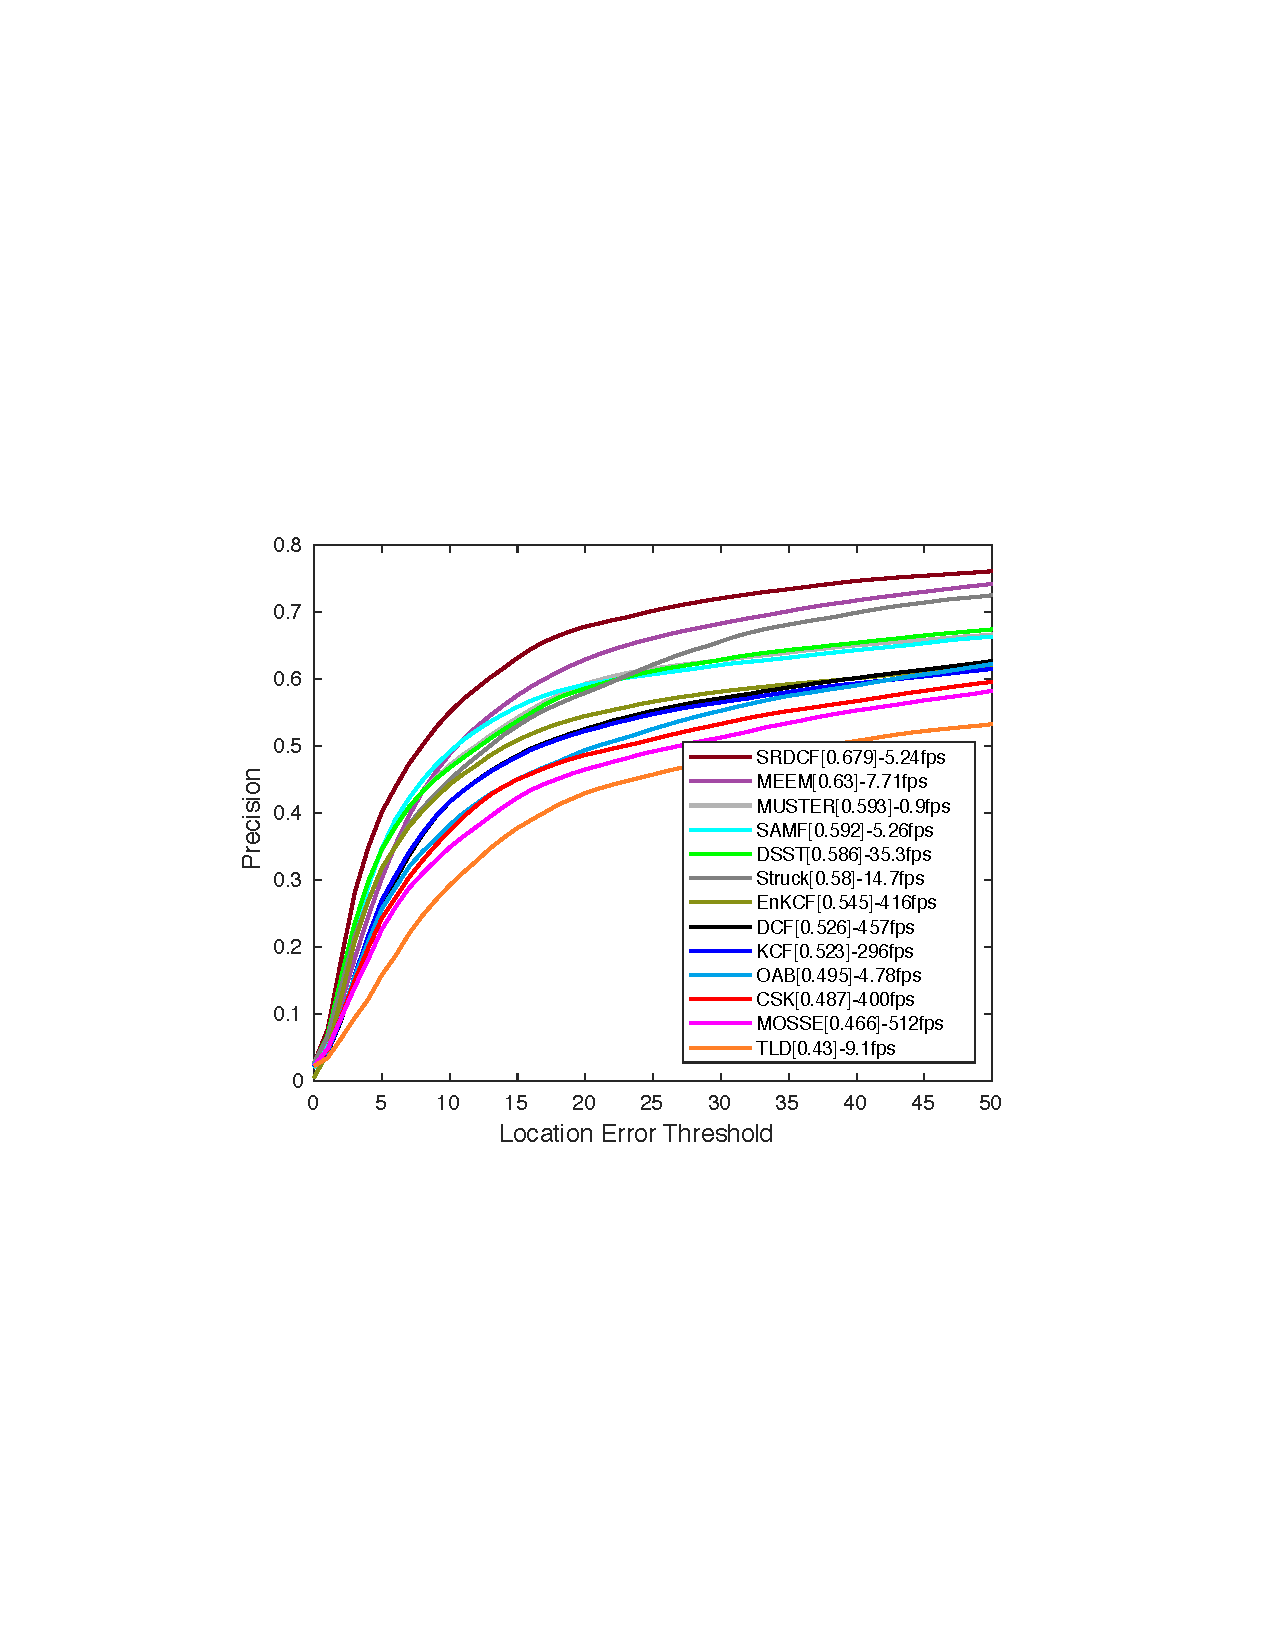
\includegraphics[width=4.00cm]{./figures/Precision_UAV123.pdf}}
\bmvaHangBox{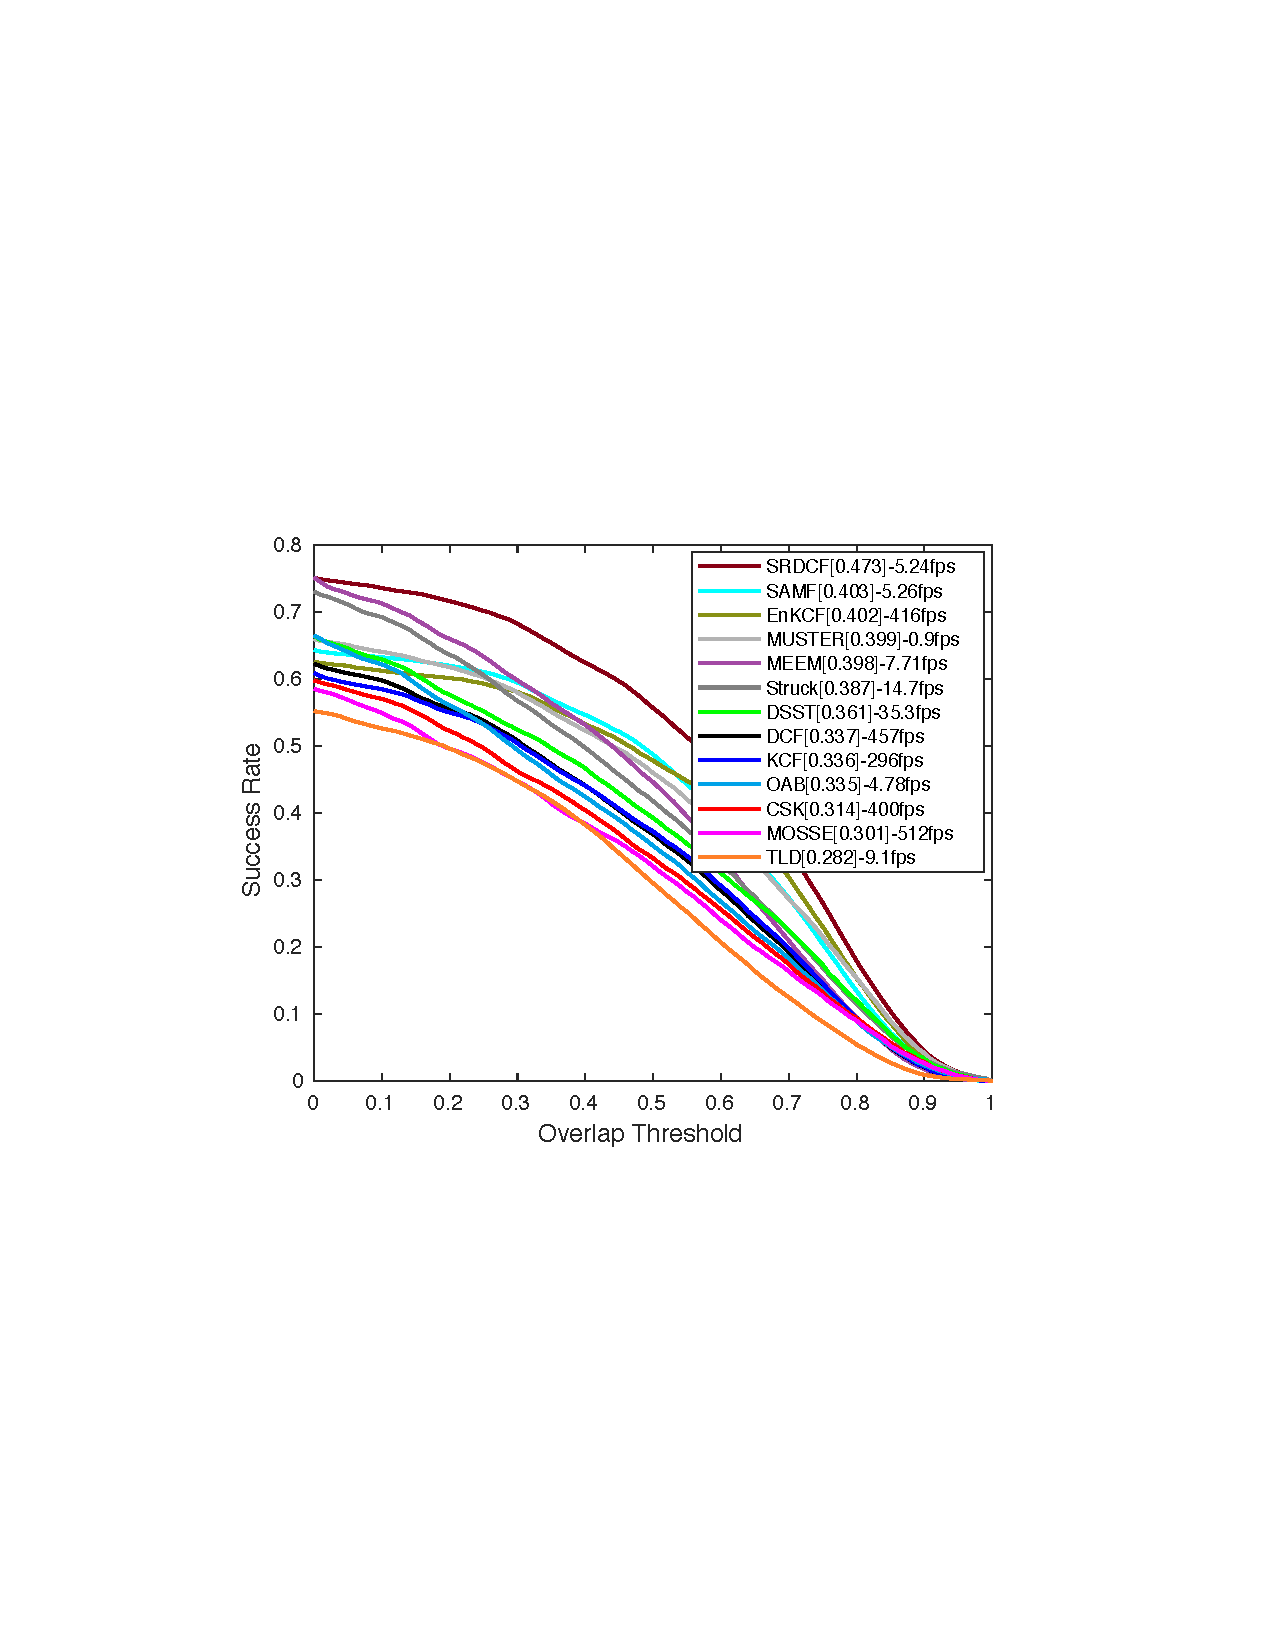
\includegraphics[width=4.0cm]{./figures/Success_UAV123.pdf}}\\
\end{tabular}
\caption{Evaluation and comparison of the proposed {\it E}nKCF tracker on the UAV123 dataset. UAV123 Dataset consists of $123$ video sequences captured from a micro UAV including large camera motion, low resolution objects, partial and full occlusions. Our tracker better fits to tracking from aerial platforms as the scale change in successive frames are not dramatic.}
\label{fig:UAV123_DATASET}
\end{figure}

\begin{figure}
\centering
\begin{tabular}{cc}
\bmvaHangBox{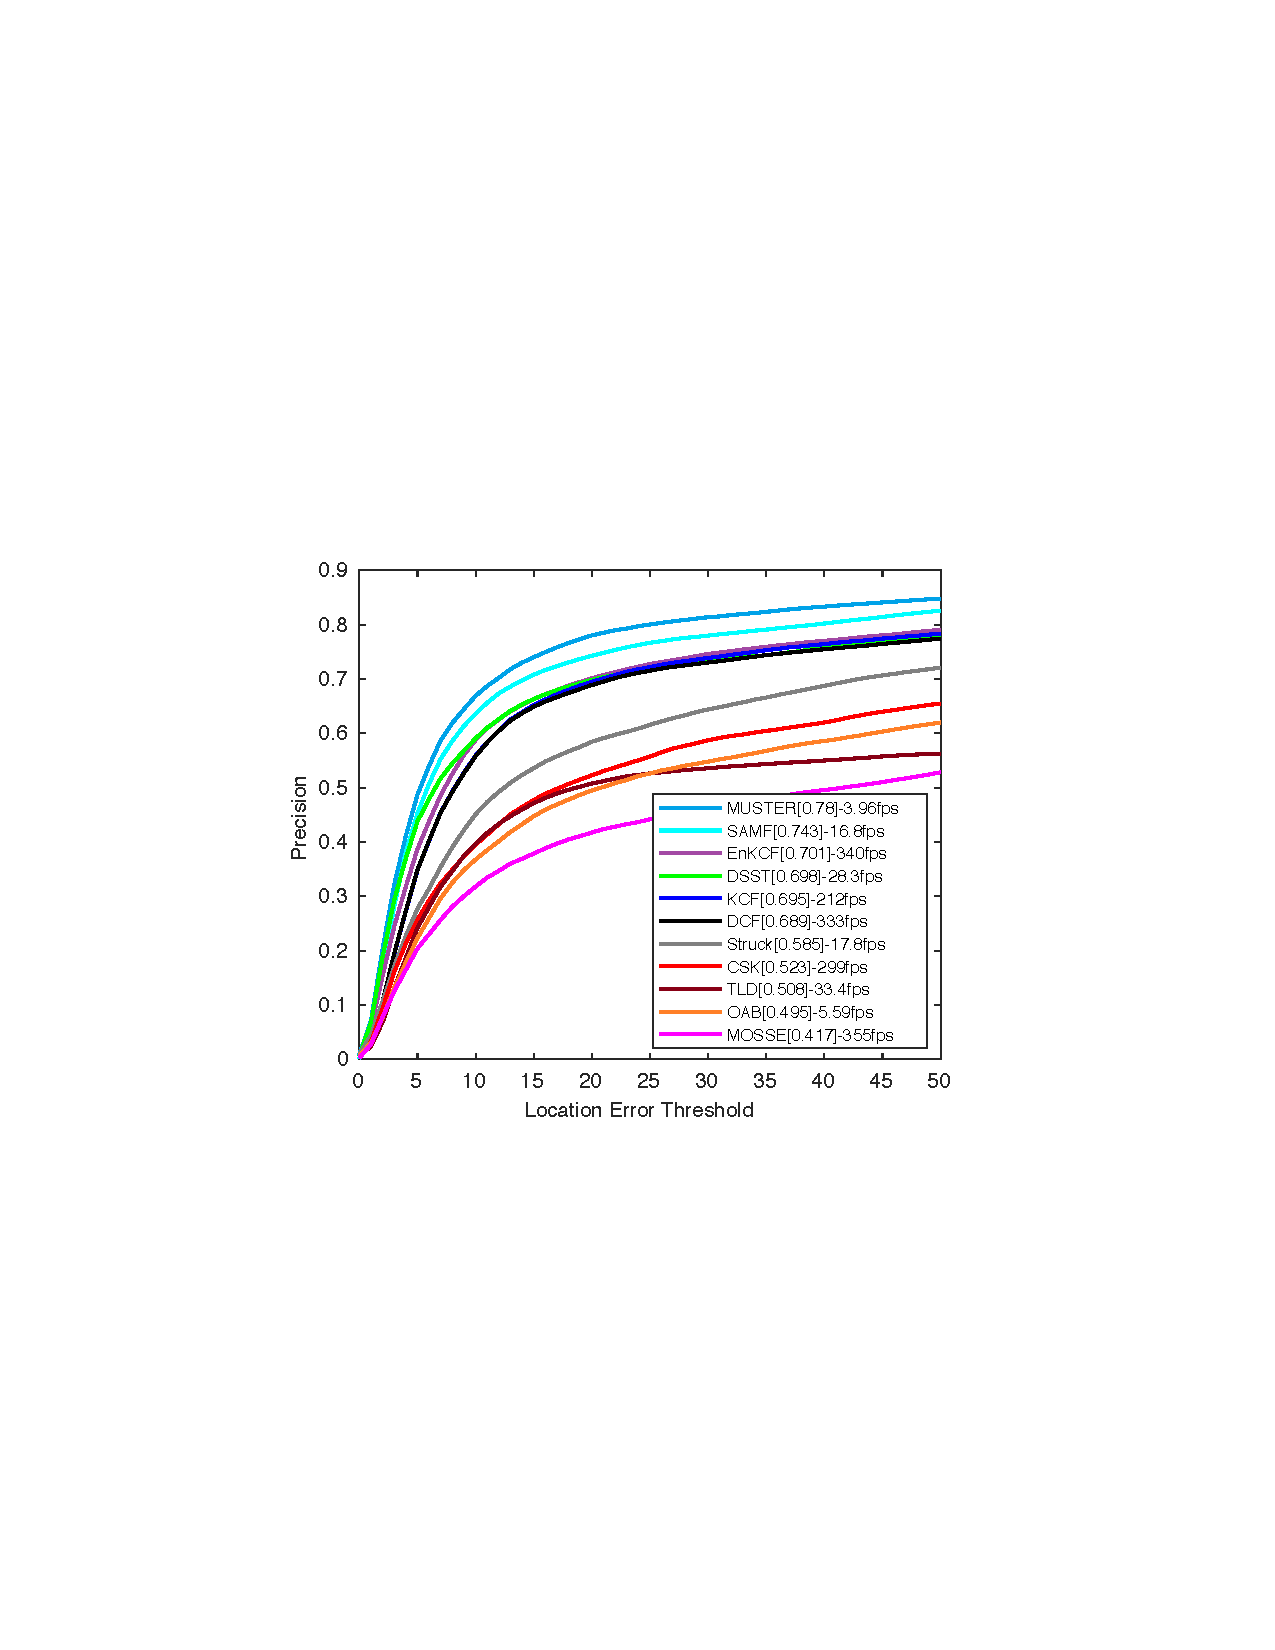
\includegraphics[width=4.00cm]{./figures/Precision_OTB100.pdf}}
\bmvaHangBox{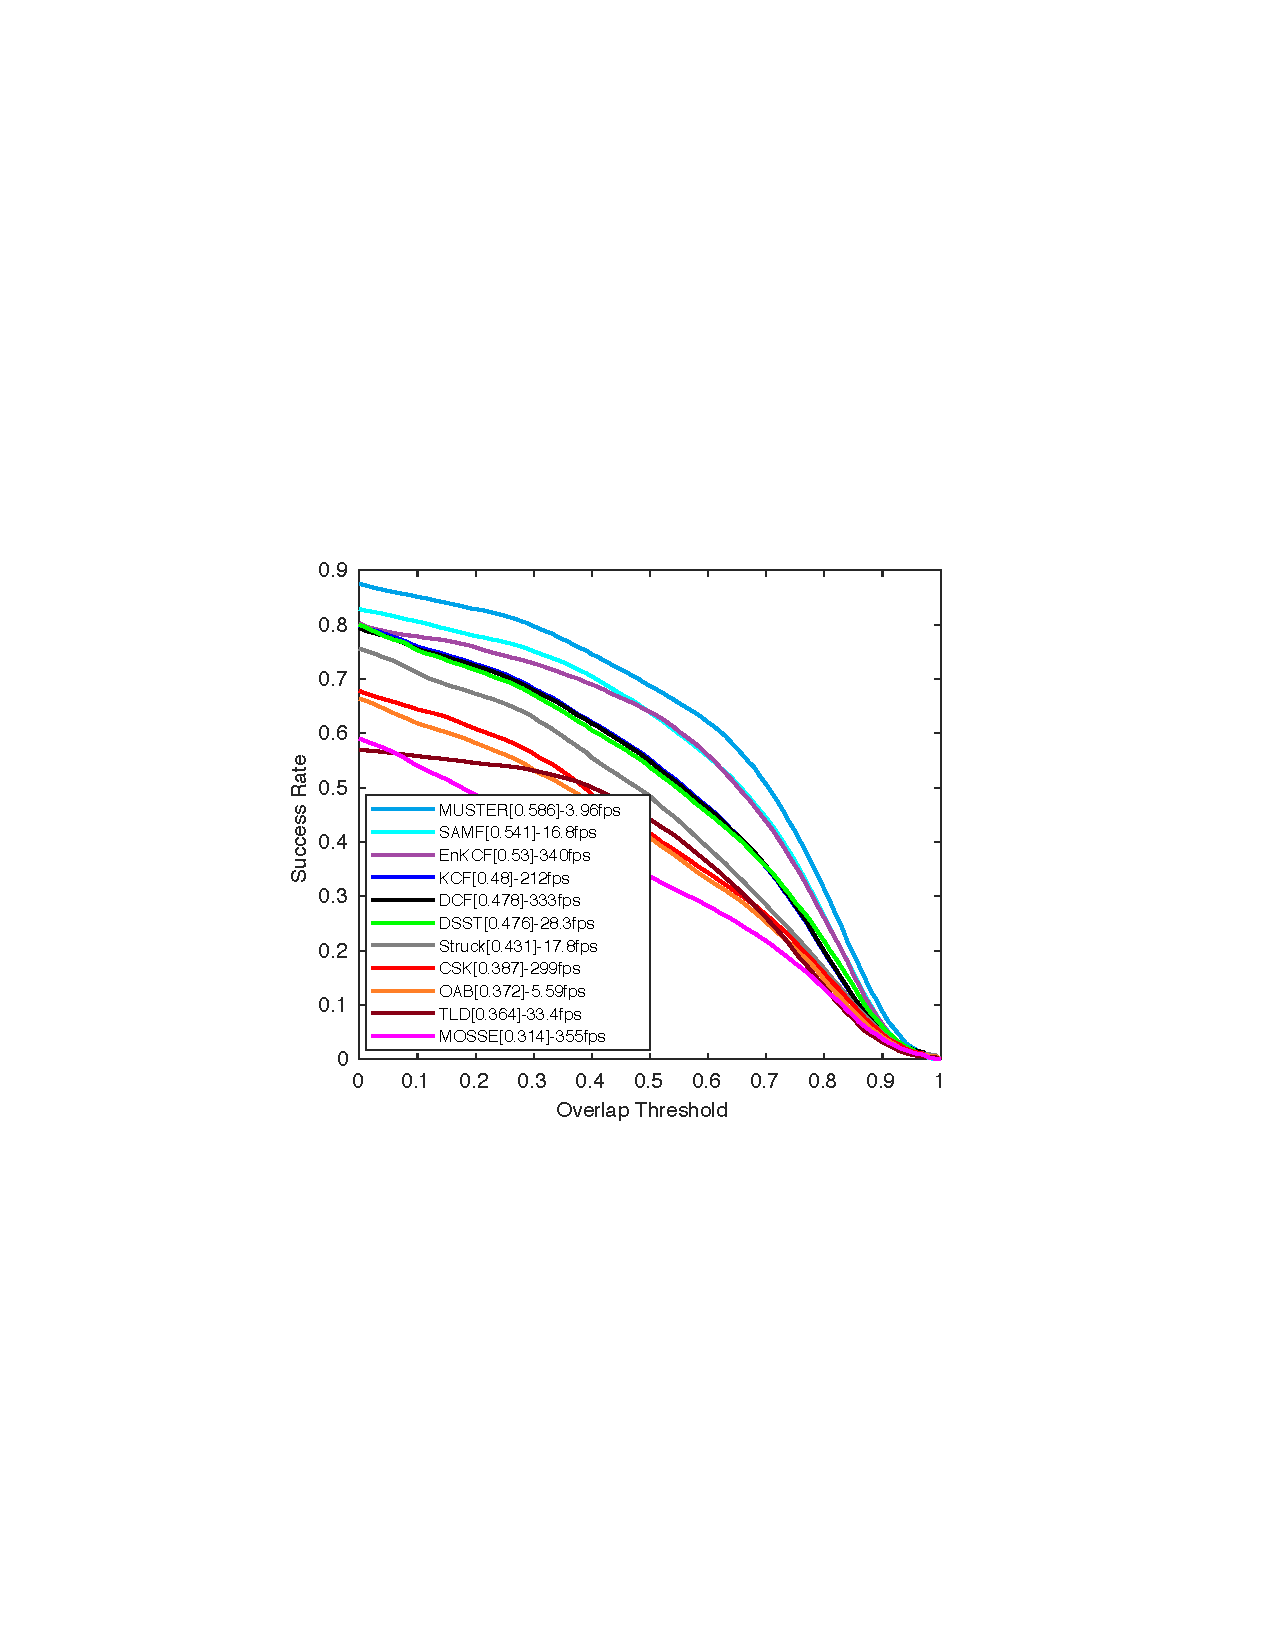
\includegraphics[width=4.0cm]{./figures/Success_OTB100.pdf}}\\
\end{tabular}
\caption{Evaluation and comparison of the proposed {\it E}nKCF tracker on the OTB100 dataset. OTB100 dataset consists of $100$ video sequences of different objects from recent literatures.}
\label{fig:OTB100_DATASET}
\end{figure}

\textbf{Performance on UAV123 Dataset.}  We compared the performance
of the proposed tracking algorithm with those of the state-of-the-art
high speed tracking algorithms in the \textit{Precision} and
\textit{Success\:Rate} metrics. Precision is computed by thresholding
the average euclidean distance between the centroid of the ground
truth and that of an tracking algorithm output. 

{\it Burak: What do mean by the following sentence? We had graphs
  about precision, but I don't see any tables or anything else to rank
  the algorithms based on the precision at 20 pixels.}

{\it YoungWoo : Trackers are ranked in the legend in the graphs - the numbers next 
to each tracker is precision at 20 px and AUC for the success rate. It is how people rank
trackers in precision and success plots. I agree with you that we can have an additional table. Let me know what
you think about it now.} 

In precision, we rank the trackers based on the precision numbers at
20 pixels. 

The success rate metric counts how many outputs from a tracking
algorithm successfully overlap with those of the ground truth greater
than a given threshold. The overlap is specifically computed by the
Intersection-Over-Union (IoU) between a tracking output and that of
the ground truth. Given the number of the correct frames based an IoU
threshod, the success rate is the ratio of the correct frames to the
number of the total frames for testing.  In the success rate plots, trackers are
ranked based on AUC scores.

{\it Burak: After you remove some of the trackers, replace that number
  with ``some'' at the below as well as removing their names from the
  following paragraph.}

{\it YoungWoo :  I thought we were going to do that tomorrow. I have generated figures and 
I can easily remove any ones. SRDCF and MEEM are the top two as of now. I am working on removing them as of now. Please 
consider that we do not have SRDCF and MEEM while you are editing the results section.}

We compare our tracker to other high-speed ($\geq$300 fps)
state-of-the-art trackers including KCF\cite{henriques2015high}, CSK
\cite{henriques2012exploiting}, STC\cite{zhang2014fast},
MOSSE\cite{bolme2010visual,henriques2015high}. Also, some relatively
lower-speed ($\geq$50) trackers are used to evaluate the robustness of
the proposed trackers. These trackers include SAMF\cite{li2014scale},
DSST\cite{danelljan2014accurate}, MEEM\cite{zhang2014meem}, Struck\cite{hare2012efficient}, and SRDCF\cite{danelljan2015learning}.
Fig.~\ref{fig:UAV123_DATASET} shows the results on the UAV123
dataset. 

{\it Burak: I will re-write the text at below after you clean up the graphs.}

{\it E}nKCF outperformed other, high-speed tracking methods by
$3\%$-$15\%$ at 20 pixels precision metric whereas it is only $5\%$
worse than SAMF, DSST and Struck on the same dataset although it is
$10$-$20$ times faster than these trackers. On the other hand, the
{\it E}nKCF does a decent job on approximating the scale of the target
in highly efficient manner. This is proved by the fact that it ranks
third best tracker in terms of \textit{area under curve} (AUC) value
for the success rate plot. It outperforms the high speed trackers by
about $20\%$-$25\%$ in AUC metric. Interestingly, it performs even
better than most of the low speed trackers. For instance, it
outperforms Struct and DSST by $5\%$ and $10\%$ while running at more
than $30$ and $10$ times larger operation rate.

\textbf{Performance on UAV123$\_$10fps Dataset.} We test our
slightly modified version of the {\it E}nKCF, {\it E}nKCF2, on the
UAV123$\_$10fps dataset. This dataset is downsampled at $10$ fps
version of the UAV123 dataset. The original dataset is already
dominated by fast object motion and large ego-motion. With
downsampling, it becomes very challenging with object and ego-motion
getting drastically larger. The performance of the proposed {\it
  E}nKCF2 tracker and other already mentioned trackers can be seen in
fig.~\ref{fig:UAV123_10fpsDATASET}. Our tracker outperforms other
high-speed correlation filter based trackers including KCF, DSST by
about $15\%$-$20\%$ whereas having similar precision rate to SAMF. On
the other hand, it does decent job in scale estimation. It ranks as
$4$th in AUC and it is $20$-$30$ faster than the ones with
higher AUC.

\begin{figure}
\centering
\begin{tabular}{cc}
\bmvaHangBox{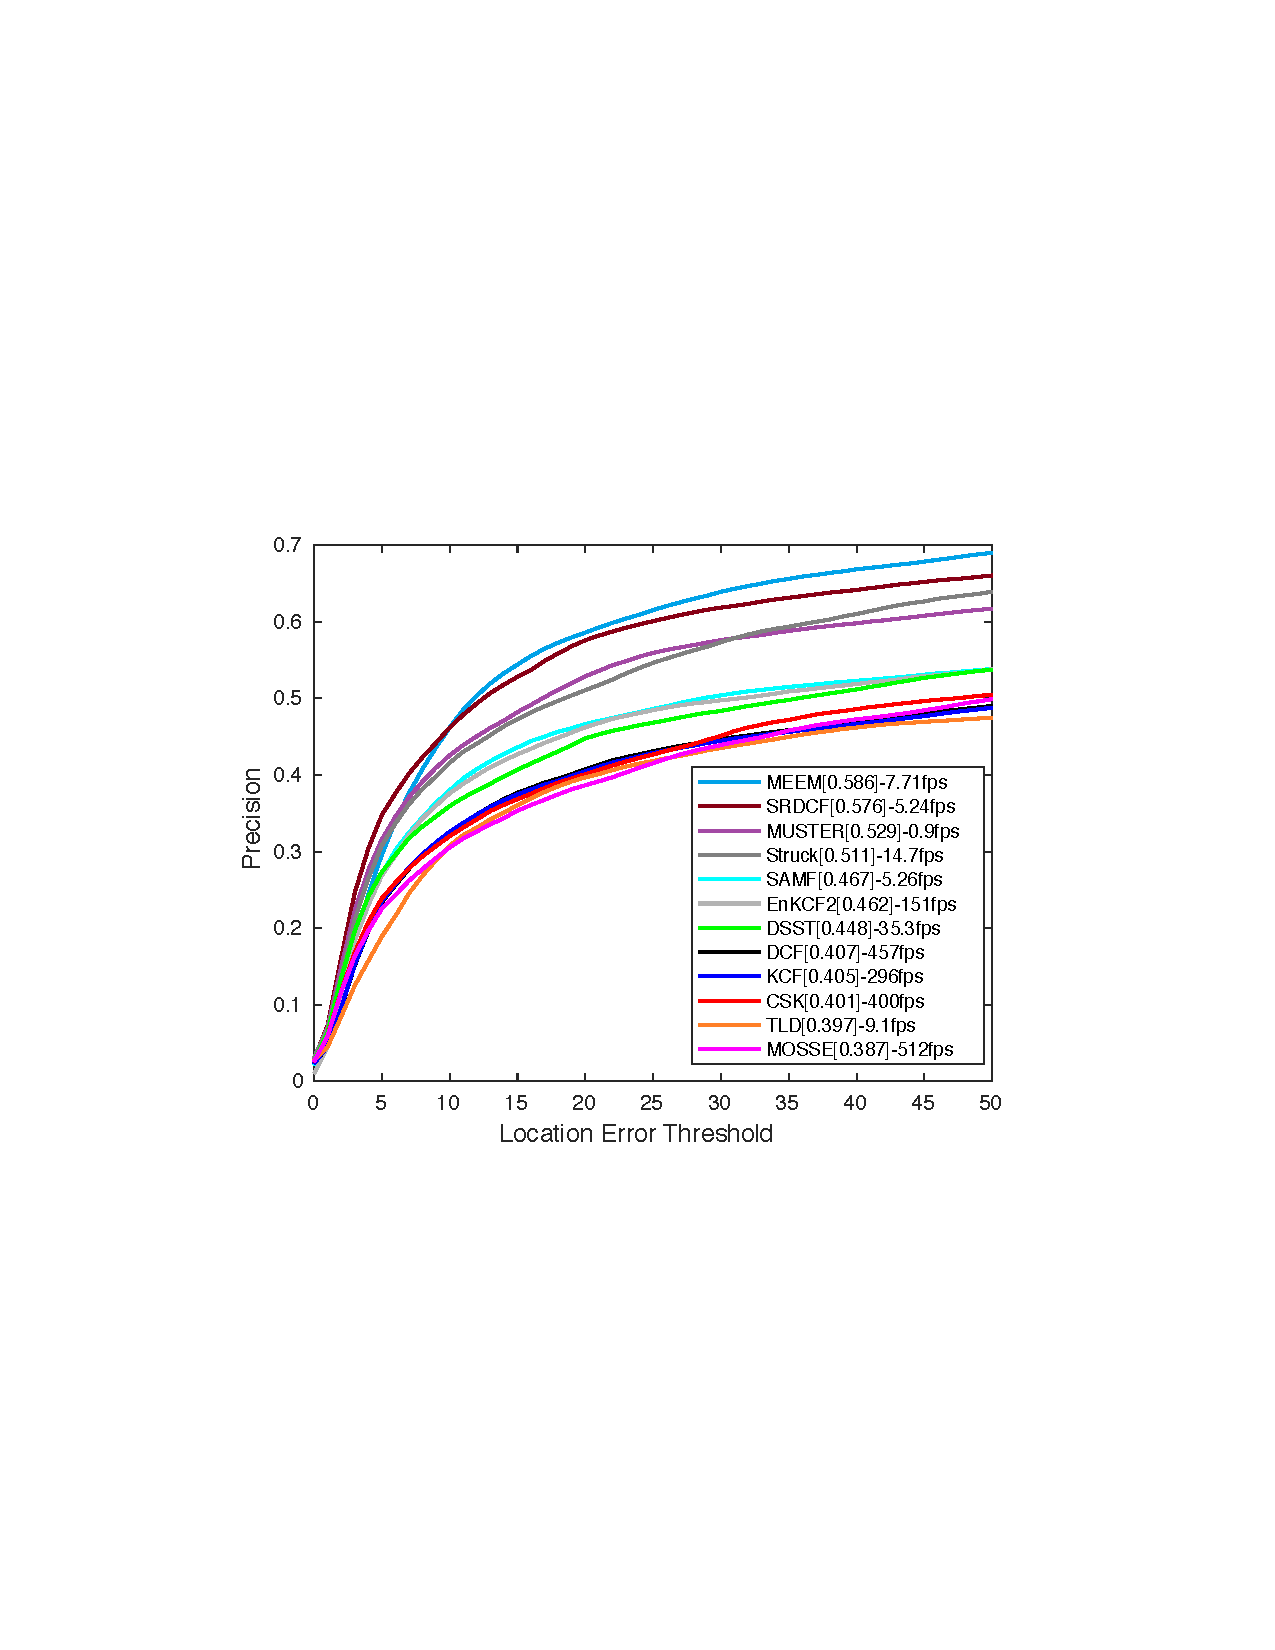
\includegraphics[width=4.00cm]{./figures/Precision_UAV123_10fps.pdf}}
\bmvaHangBox{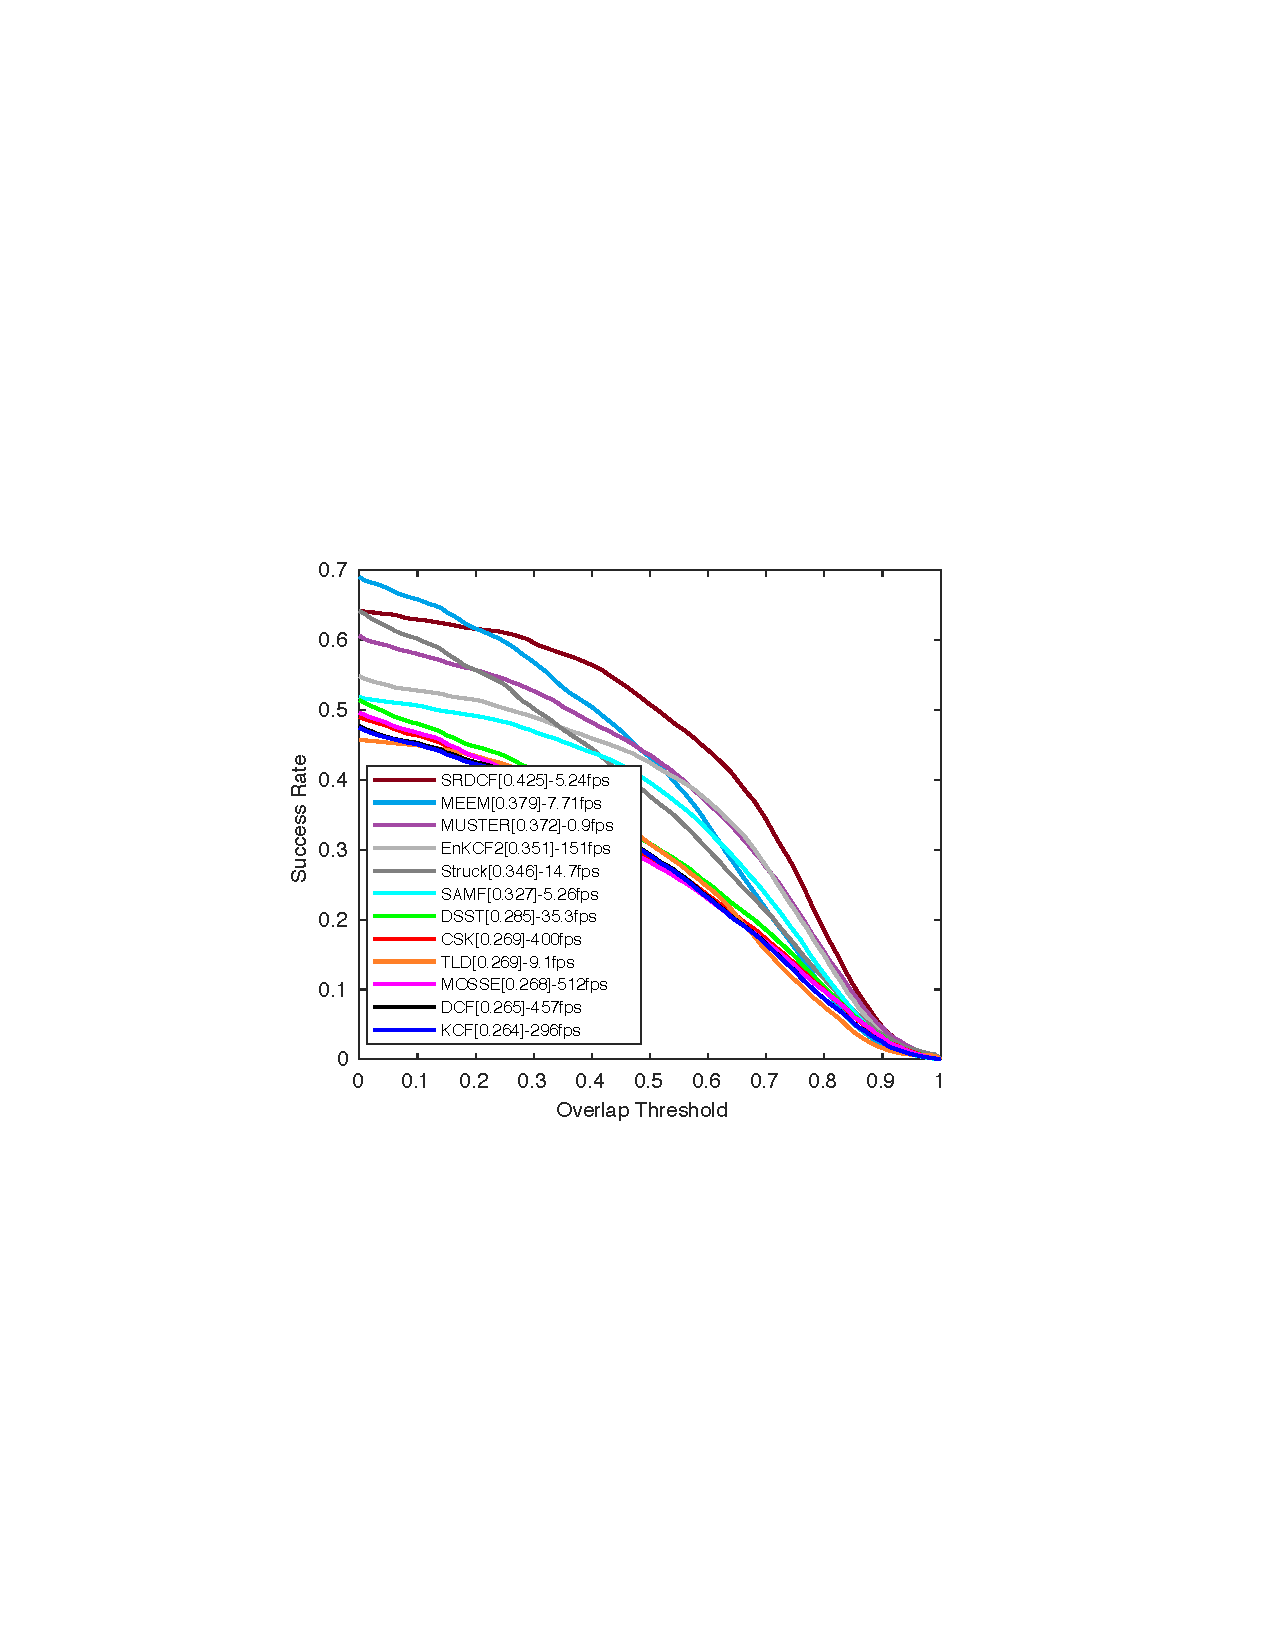
\includegraphics[width=4.0cm]{./figures/Success_UAV123_10fps.pdf}}\\
\end{tabular}
\caption{Evaluation and comparison of the proposed {\it E}nKCF2 tracker on the UAV123$\_$ dataset in terms of the precision and success rates. This dataset consists of temporally downsampled $123$ video sequences captured from a micro UAV.}
\label{fig:UAV123_10fpsDATASET}
\end{figure}

\textbf{Performance on OTB100 Dataset.}
In addition to UAV123 dataset, we test the {\it E}nKCF tracker on the
OTB100 dataset to evaluate how good it generalizes to a traditional
object tracking dataset. Again, it performs slightly better than the
high speed trackers in precision. Interestingly, it outperforms the
another correlation filter based tracker, DSST while running only
$5\%$ behind of another low-speed scale adaptive SAMF tracker. As in
UAV123 dataset, the {\it E}nKCF performs exceptionally in handling the
scale changes. It is ranked as the fifth best tracker while being the
second highest speed tracker behind MOSSE. It performs only around
$2\%$ worse than SAMF and MEEM trackers in terms of AUC. These numbers
prove that {\it E}nKCF is not only a good candidate for tracking on a
UAV-based mobile platform but also mobile platforms on smart phones.

%---------------------------------------------------------------------- 
\section{Conclusion} \label{sc:Conclusion}
%---------------------------------------------------------------------- 

%--------------
%\section*{Acknowledgements}
%put stuff here for the accepted , but not the ICCV version

\bibliography{draft}
\end{document}
